\documentclass[acmlarge,screen]{acmart}

\acmJournal{DGOV}
\acmVolume{0}
\acmNumber{0}
\acmArticle{0}
\acmYear{2026}
\acmMonth{9}
\acmDOI{XX.XXXX/XXXXXXX}

\setcopyright{none}
\renewcommand\footnotetextcopyrightpermission[1]{}
\settopmatter{printacmref=false}

\usepackage{booktabs}
\usepackage{graphicx}
\usepackage{xcolor}
\usepackage{amsmath}

\title{Grouping Duplicate Citizen Complaints in a State Ombudsman}
\subtitle{An operational account from Cear\'{a}, Brazil}

\author{Berg Silva}
\affiliation{%
  \institution{Controladoria e Ouvidoria Geral do Estado do Cear\'{a} (CGE-CE)}
  \city{Fortaleza}
  \country{Brazil}}

\author{Charles}
\affiliation{%
  \institution{Controladoria e Ouvidoria Geral do Estado do Cear\'{a} (CGE-CE)}
  \city{Fortaleza}
  \country{Brazil}}

\author{Ana Luiza Cruz}
\affiliation{%
  \institution{Controladoria e Ouvidoria Geral do Estado do Cear\'{a} (CGE-CE)}
  \city{Fortaleza}
  \country{Brazil}}

\author{Francisco Nauber Bernardo Gois}
\authornote{Corresponding author.}
\affiliation{%
  \institution{Controladoria e Ouvidoria Geral do Estado do Cear\'{a} (CGE-CE)}
  \city{Fortaleza}
  \country{Brazil}}
\email{francisco.gois@cge.ce.gov.br}

\renewcommand{\shortauthors}{Silva et al.}

\begin{CCSXML}
<ccs2012>
 <concept>
  <concept_id>10010405.10010455.10010459</concept_id>
  <concept_desc>Applied computing~Computing in government</concept_desc>
  <concept_significance>500</concept_significance>
 </concept>
 <concept>
  <concept_id>10002951.10003317.10003347.10003350</concept_id>
  <concept_desc>Information systems~Clustering and classification</concept_desc>
  <concept_significance>300</concept_significance>
 </concept>
 <concept>
  <concept_id>10010147.10010178.10010179</concept_id>
  <concept_desc>Computing methodologies~Natural language processing</concept_desc>
  <concept_significance>300</concept_significance>
 </concept>
</ccs2012>
\end{CCSXML}

\ccsdesc[500]{Applied computing~Computing in government}
\ccsdesc[300]{Information systems~Clustering and classification}
\ccsdesc[300]{Computing methodologies~Natural language processing}

\keywords{citizen complaints, ombudsman, near-duplicate detection, text clustering, sentence embeddings, HDBSCAN, digital government, Brazil}

\begin{abstract}
A citizen can tell the same story ten times in one morning. Each wording looks like a new file. The officer reads the pile twice, and the person who wrote waits.

Similaridade is the grouping job used by the Controladoria e Ouvidoria Geral do Estado do Cear\'{a} (CGE-CE). It asks whether two free-text complaints point to the same event. On one historical batch of 4{,}389 real complaints, the production stack (TF-IDF + DBSCAN, keep a group if mean intra-cluster cosine similarity $\ge 0.75$) grouped 62.4\% of the texts. The same batch, encoded with sentence embeddings and clustered with HDBSCAN, grouped an inferred 82.5\% before any language model. Adding a leftover pass through DeepSeek R1 raised the reported share to 84.9\% (3{,}725 complaints). That last step recovered 104 of 768 leftovers after seeing only 27 candidates. How those 27 were chosen is not in the team note. Whether the model ran inside CGE is also unknown. We therefore treat 84.9\% as an ablation with an undocumented filter, not as a deployment result.

None of these rates is a precision. The Ouvidoria has not labeled a sample of ``same case.'' The same production rule, replayed on downloaded public packs, grouped 3.2\% of a 20~Newsgroups slice, 17.0\% of BBC News, and 10.5\% of a Reuters single-topic slice. In September 2026 the live job at times collapsed to a single cluster. The claim that survives is smaller: lexical clustering already catches copy-paste waves; a semantic stack grouped more of the same historical set; daily production of that stack, and any leftover language-model path, is still being earned.
\end{abstract}

\begin{document}
\maketitle

\begin{quote}
\small\textit{Draft v0.5 --- 24 September 2026. Practice paper aimed at ACM DGOV, not submitted. Authorship is provisional. Figures: Grok Imagine scene; rates and labels typeset from team counts. Prior Sonar read: \texttt{docs/perplexity-review.md}. Venue note: \texttt{docs/journal.md}.}
\end{quote}

\begin{figure*}[t]
\centering
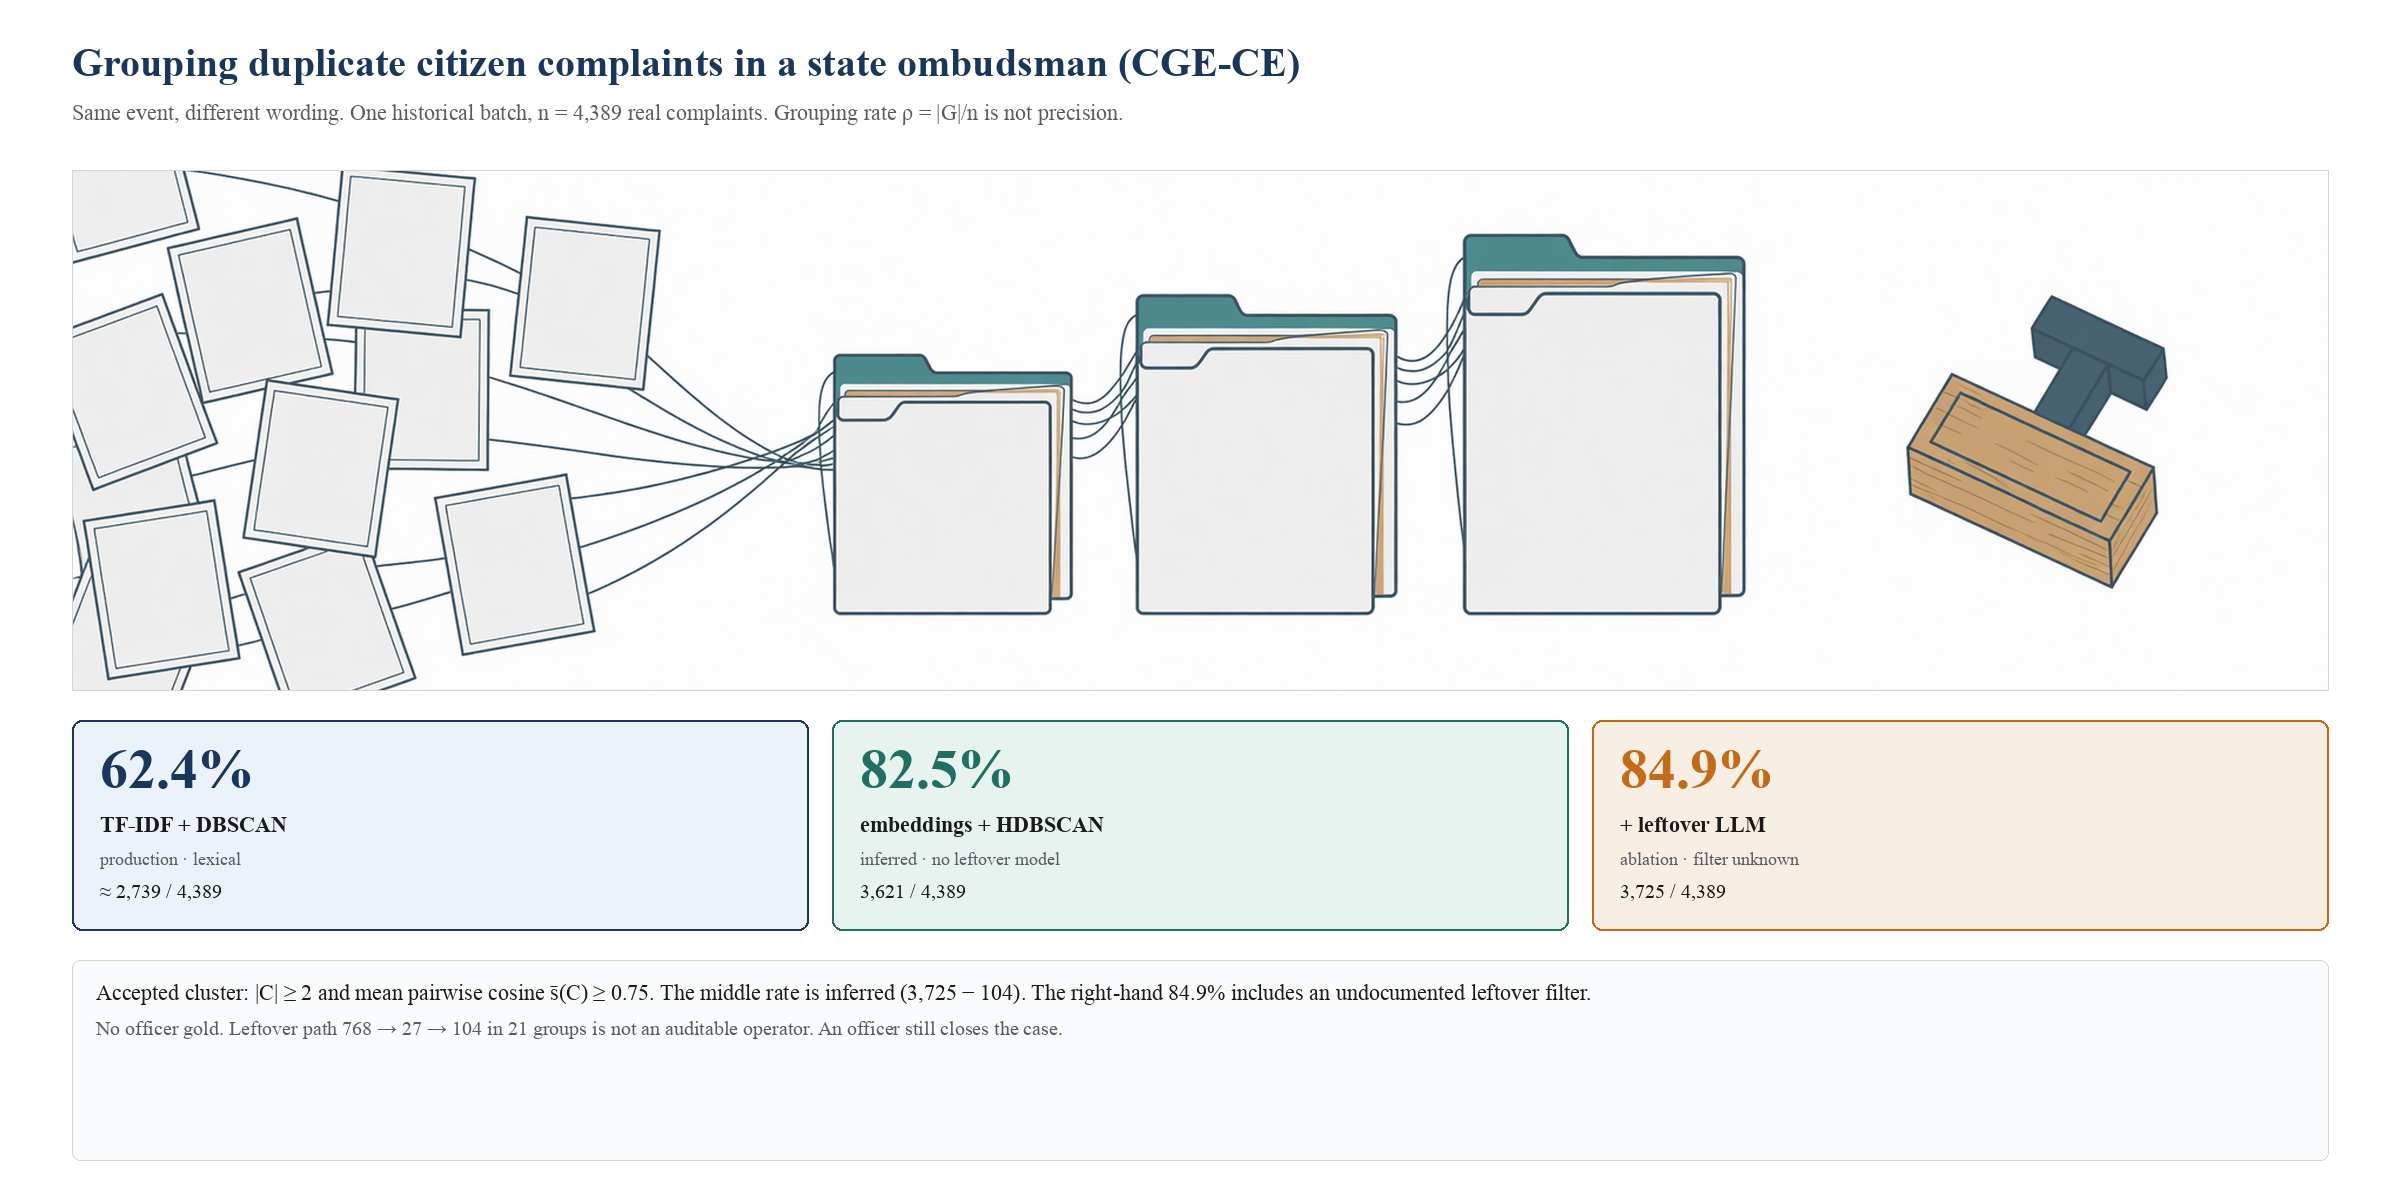
\includegraphics[width=\textwidth]{figures/fig_abstract.png}
\caption{Graphical abstract. Scene drawn with Grok Imagine; rates and the acceptance rule typeset from the team note. $\rho$ is a grouping rate, not precision. The leftover language-model step is an ablation.}
\label{fig:teaser}
\end{figure*}

\section{Introduction}

An ombudsman file starts as free text. The same broken pipe, the same delay at a public counter, or the same coordinated campaign can arrive tens of times before lunch. If each arrival becomes its own case, the officer repeats the same reading and the citizen waits longer (Figure~\ref{fig:teaser}).

Similaridade sits on the complaint stream of the state Ouvidoria (COUVI). The job is narrow. Put texts that likely refer to the same event in one group. Mark the rest as leftovers. Show the officer a provisional review queue---green, yellow, red---instead of a raw list.

Most public-sector NLP work classifies a complaint into a department or extracts a theme~\cite{das2020grievance,tang2024bertopic,rakhimzhanov2025transport,silva2026bridging}. Similaridade is closer to near-duplicate detection~\cite{broder1997resemblance,rabbi2026duplicate}: it asks whether two texts are the same case. TF-IDF, DBSCAN, sentence transformers, and HDBSCAN are known tools~\cite{salton1988term,ester1996dbscan,reimers2019sbert,campello2013hdbscan}. What this draft can still offer is an operational account: one Brazilian state stream, three treatments on the same 4{,}389 complaints, a conservation table that does not fully close, and a protocol for the labels that are still missing.

Four questions stay after the August tests.
\begin{enumerate}
\item How much of a real complaint batch does lexical clustering already group?
\item How much more does embedding + HDBSCAN group on the same batch, before any language model?
\item What does the leftover language-model pass add, and what must be known before that add is credited?
\item What still breaks when the job runs every day?
\end{enumerate}

This version does not invent officer labels, clustering radii, or a model name. Where the team note is silent, the table says unknown.

The first venue for this draft is ACM \textit{Digital Government: Research and Practice} (DGOV), practice track. The paper is an operational account, not a new clustering theorem. Method journals would ask for a gold partition we do not have.

\section{State of the art}

Public grievance research splits into three jobs that are easy to mix up. Figure~\ref{fig:case} is the cut that matters for an ombudsman officer.

\begin{figure*}[t]
\centering
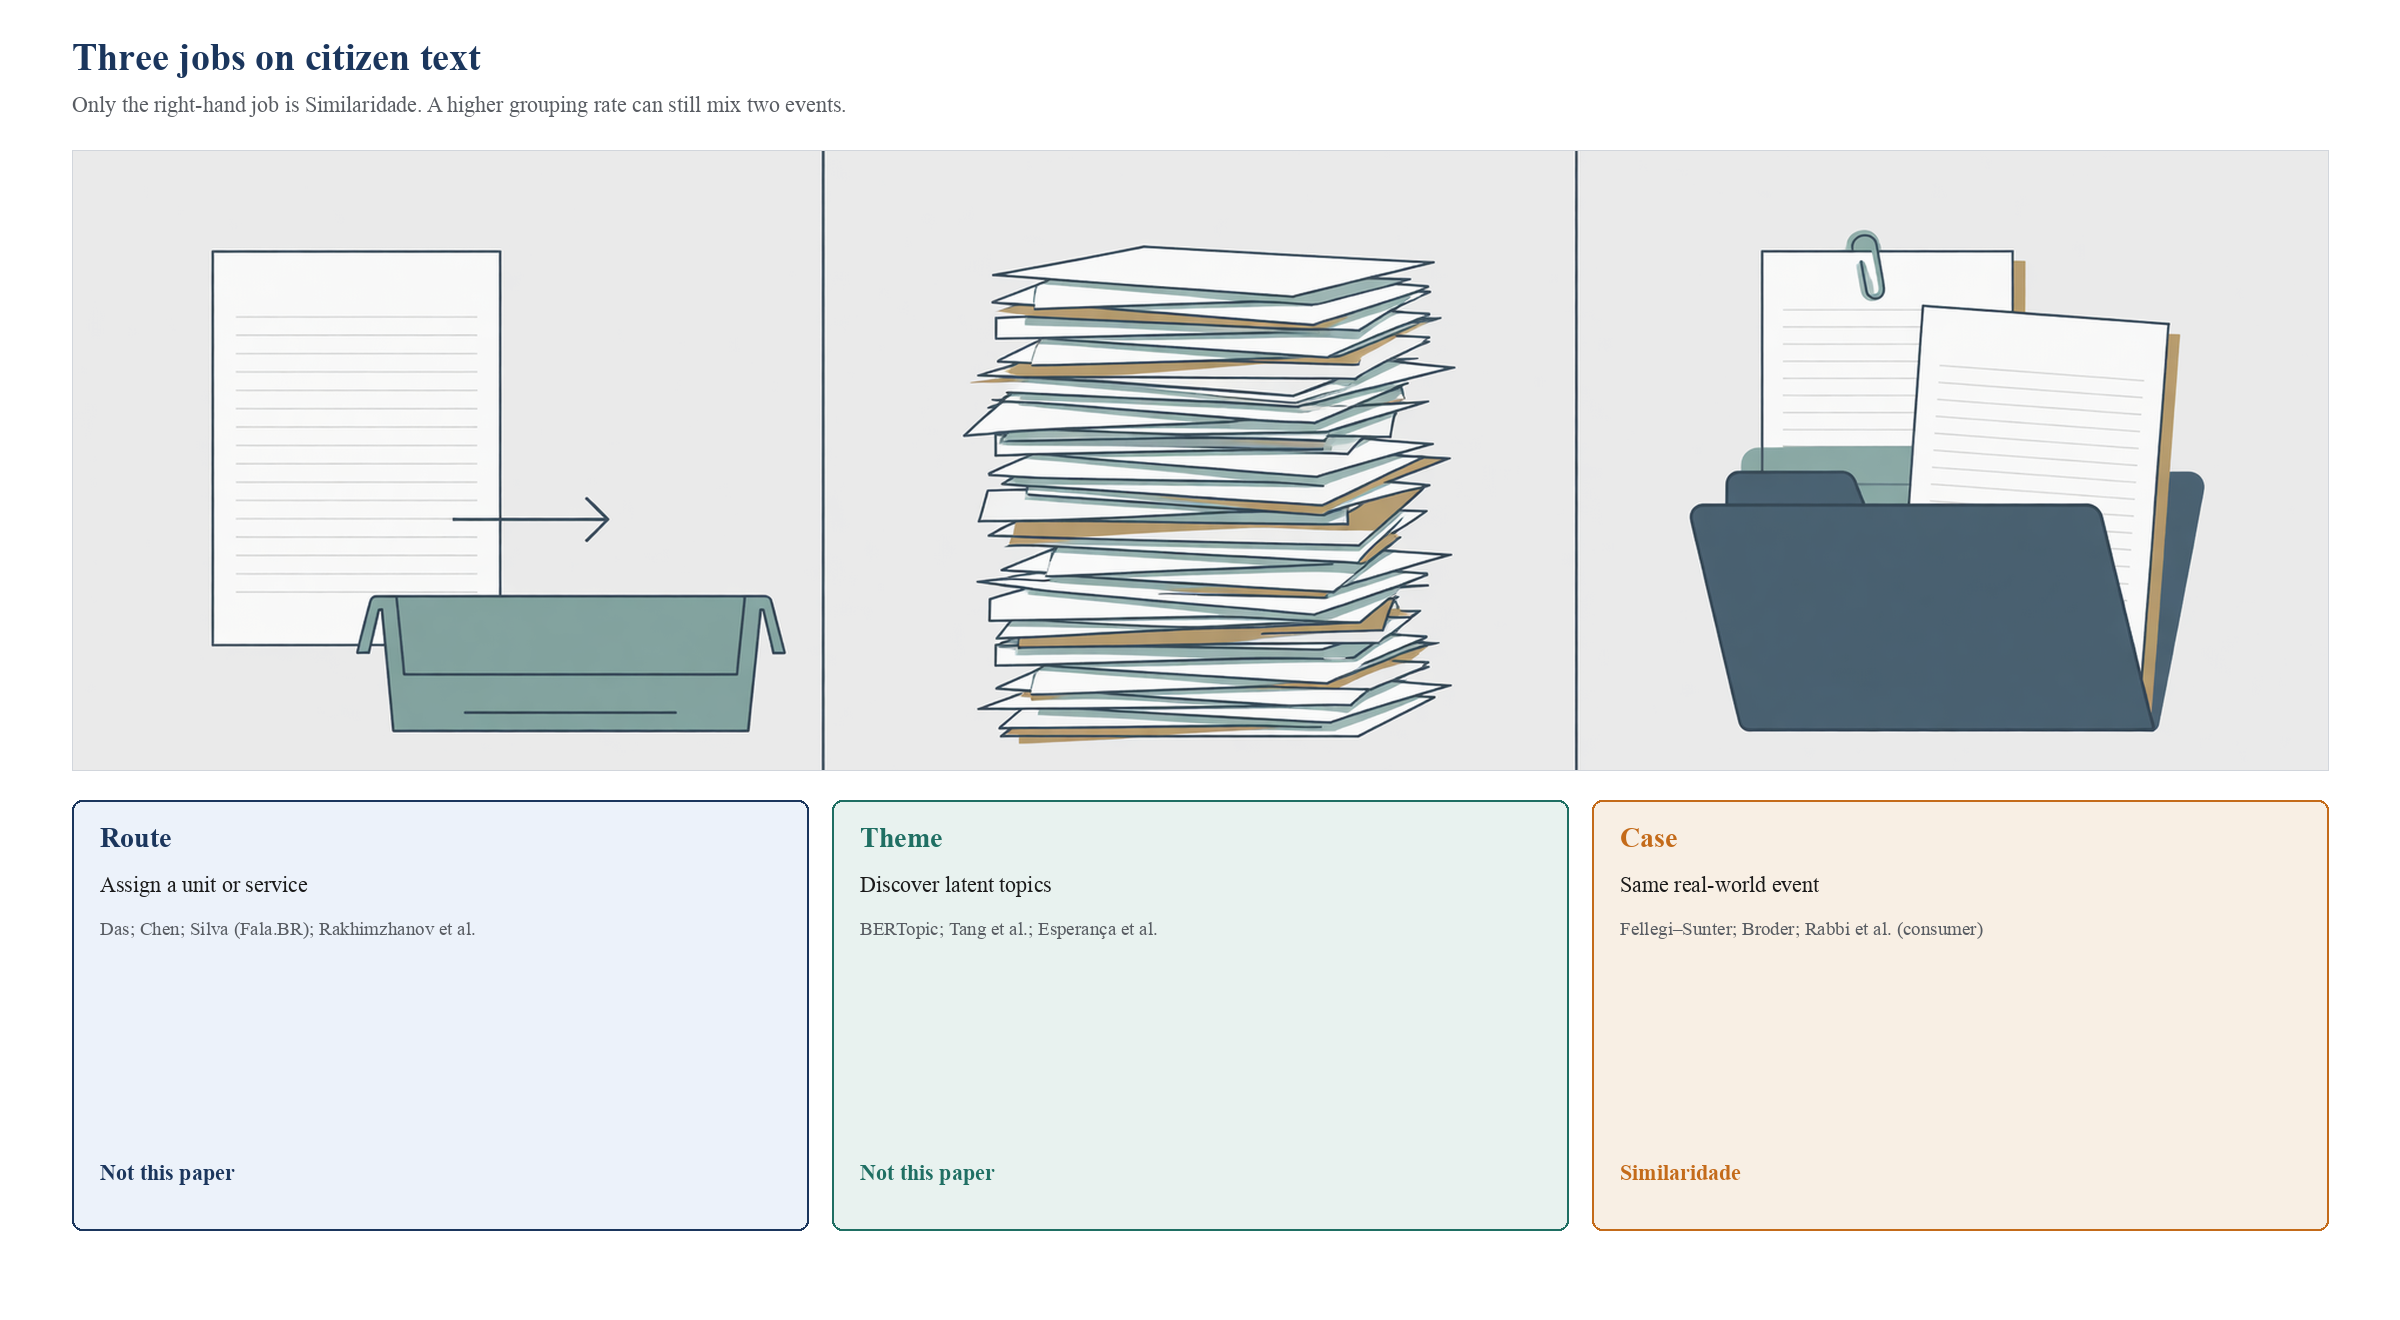
\includegraphics[width=0.92\textwidth]{figures/fig_jobs.png}
\caption{Three jobs on citizen text. Route assigns a unit. Theme discovers a topic. Case groups the same event. Only the third job is Similaridade. Scene: Grok Imagine; labels set in type.}
\label{fig:case}
\end{figure*}

\paragraph{Routing and classification.}
A first line assigns a complaint to a unit or a service. Das et al.\ used sentence-level sentiment to help officers triage incoming text~\cite{das2020grievance}. Rakhimzhanov, Belginova, and Yedilkhan compared large language models with instruction-tuned embeddings on municipal transport complaints; fine-tuned embeddings reached about 90\% accuracy and were cheaper than prompting an LLM for every item~\cite{rakhimzhanov2025transport}. Silva et al.\ linked Brazilian federal ombudsman manifestations on Fala.BR to official public services with BM25 and dense retrieval plus RAG-expanded labels~\cite{silva2026bridging}. That is routing. Two texts about the same water outage can share a service and still be two cases, or two services and still be one case.

\paragraph{Theme discovery.}
A second line asks what citizens talk about. BERTopic embeds documents, reduces them, clusters with HDBSCAN, and labels each cluster with class-based TF-IDF~\cite{grootendorst2022bertopic}. Tang, Pan, and Gu used that recipe on China's online government inquiry platform~\cite{tang2024bertopic}. Theme models help policy. They are the wrong metric when an officer must link a copy-paste wave that shares one event and many wordings.

\paragraph{Duplicate and same-event grouping.}
A third line asks whether two records are the same complaint or the same event. That is record linkage and duplicate detection, not topic modelling~\cite{fellegi1969linkage,elmagarmid2007duplicate}. Broder's resemblance test did the job for web pages~\cite{broder1997resemblance}. Rabbi et al.\ did it for Portuguese consumer complaints across Consumidor.gov.br, Procon, and Sindec: BERTimbau embeddings~\cite{souza2020bertimbau}, a cosine threshold set with domain experts (90\% in their study), and a 30-day window. Most of their duplicates arrived inside that window~\cite{rabbi2026duplicate}. Their unit is often the same consumer repeating a claim. An ombudsman wave can also be many people writing one outage. Esperan\c{c}a et al.\ clustered informatics complaints in a Portuguese public agency so repeated issues surface once; the target is still a category~\cite{esperanca2025complaint}. The closest public gold for ``same question, different wording'' is CQADupStack, twelve StackExchange sites with duplicate-thread labels~\cite{hoogeveen2015cqadupstack}. News and social streams treat the same cut as first-story or event detection: TDT asked for the first story of an event~\cite{allan1998tdt}; Petrovi{\'c}, Osborne, and Lavrenko scaled that job to Twitter~\cite{petrovic2010fsd}; McMinn, Moshfeghi, and Jose released Events~2012 with more than 500 crowd-judged events~\cite{mcminn2013events}. Those corpora are the right family. 20~Newsgroups is not: Lang's collection is a topic filter, not an event partition~\cite{lang1995newsweeder}. Romberg and Escher, writing in DGOV itself, treat duplicate detection as one of three evaluation jobs on citizen text, and they name the same gaps we still have: quality of the groups, non-English corpora, and a tool an officer can actually run~\cite{romberg2023citizens}. Chen et al.\ turn government complaints into a classification problem so a server can route a reply~\cite{chen2022igcp}. That is still routing. Similaridade does not pick a department. It asks whether two files should share one case.

\paragraph{Where Similaridade sits.}
Table~\ref{tab:sota} places the stacks against that map. Production Cear\'{a} is lexical near-duplicate detection on short state-ombudsman texts, without the identity keys and time window Rabbi et al.\ could use. The homolog stack is embeddings + HDBSCAN, plus an optional leftover language model. It is not a BERTopic run: there is no class-based TF-IDF topic label on the main clusters. What this draft still lacks is a human label of ``same case.'' Without that label, a higher grouping rate can just mean a more permissive merge. The metric that would decide the argument is BCubed precision and recall against officer gold~\cite{amigo2009bcubed}, not the share of texts placed in some group.

\begin{table}[t]
\caption{Public-sector complaint work versus Similaridade. Theme = latent topic. Route = department or service. Case = same event.}
\label{tab:sota}
\small
\begin{tabular}{p{3.4cm}p{2.4cm}p{3.1cm}p{3.0cm}}
\toprule
Work & Task & Representation & Grouping \\
\midrule
Fellegi and Sunter~\cite{fellegi1969linkage} & Record link & Field agreement & Likelihood ratio \\
Elmagarmid et al.~\cite{elmagarmid2007duplicate} & Duplicate record & Survey & Pair classifiers \\
Romberg and Escher~\cite{romberg2023citizens} & Dupl.\ / theme / argument & Review (DGOV) & Mixed NLP \\
Chen et al.~\cite{chen2022igcp} & Route / reply & Text classifier & Supervised \\
Das et al.~\cite{das2020grievance} & Route / triage & Sentiment features & Supervised \\
Tang et al.~\cite{tang2024bertopic} & Theme & Embeddings & BERTopic \\
Rakhimzhanov et al.~\cite{rakhimzhanov2025transport} & Route & E5 / BGE / LLM & Classifier \\
Silva et al.~\cite{silva2026bridging} & Route (service) & BM25 + dense + RAG & Retrieval \\
Esperan\c{c}a et al.~\cite{esperanca2025complaint} & Theme / pattern & BERT embeddings & Semantic clusters \\
Rabbi et al.~\cite{rabbi2026duplicate} & Duplicate & BERTimbau & Threshold + 30 days \\
Hoogeveen et al.~\cite{hoogeveen2015cqadupstack} & Duplicate question & cQA threads & Retrieval / pair \\
Allan et al.~\cite{allan1998tdt} & First story / event & News stream & TDT tasks \\
McMinn et al.~\cite{mcminn2013events} & Same event (tweets) & Events 2012 & Crowd events \\
Lang~\cite{lang1995newsweeder} & Theme (newsgroup) & 20 Newsgroups & Topic labels \\
Greene and Cunningham~\cite{greene2006bbc} & Theme (news) & BBC News & Topic labels \\
Lewis~\cite{lewis1997reuters} & Theme (wires) & Reuters-21578 & Topic labels \\
Wang et al.~\cite{wang2018glue} & Duplicate question & Quora (GLUE QQP) & Pair label \\
Similaridade (production) & Case & TF-IDF & DBSCAN \\
Similaridade (no LLM) & Case & Sentence embeddings & HDBSCAN \\
Similaridade (leftover LLM) & Case / theme? & Prompt on leftovers & Filter unknown \\
\bottomrule
\end{tabular}
\end{table}

On the method side the genealogy is short. Term weights still catch identical paste~\cite{salton1988term}. DBSCAN finds dense regions and treats sparse points as noise~\cite{ester1996dbscan,schubert2017dbscan}. That matches an ombudsman day: one campaign, or many singletons. The price is a fixed radius. HDBSCAN drops that radius~\cite{campello2013hdbscan,mcinnes2017hdbscan}. Sentence-BERT gives vectors that cosine can compare without a cross-encoder on every pair~\cite{reimers2019sbert}. Portuguese checkpoints exist~\cite{souza2020bertimbau}. This draft does not yet name the checkpoint that ran.

\section{Setting}

CGE-CE is the state controller and ombudsman of Cear\'{a}. Similaridade serves the Ouvidoria. ASESI builds and runs the software. Airflow starts the job. Counts later land in an internal log table (\texttt{etl.similaridade\_log}: complaints processed, grouped, leftovers, largest and smallest cluster, intra-cluster similarity).

The production schedule in August 2026 was three runs per day: 08:00, 12:00, and 17:00. Source code lives on the state's GitLab, project \texttt{analise\_similaridade\_dev}. This public draft does not copy that repository.

The 4{,}389-complaint homolog batch was reported to the team on 28 August 2026. The note does not give the extraction window, language mix, length histogram, or agency mix. Complaint text is sensitive. We report only aggregate counts already shared inside the team. No complaint body is reproduced.

\section{Definitions and counting}

The words below are operational, not legal.

\begin{itemize}
\item \textbf{Complaint.} One incoming free-text record in the batch.
\item \textbf{Cluster.} A set of complaints that the algorithm labeled together.
\item \textbf{Grouped.} A complaint in an accepted cluster of size $\ge 2$.
\item \textbf{Leftover.} A complaint not grouped after that stack's clustering step.
\item \textbf{Candidate.} A leftover passed to the language model.
\item \textbf{Recovered.} A leftover that the language model placed in a group the team later counted as grouped.
\item \textbf{Theme (leftover path).} The team's word for a leftover group returned by the language model. It may be a topic, not a same-event case.
\item \textbf{Band.} A provisional review queue (green / yellow / red). Not a measured safety threshold.
\end{itemize}

Table~\ref{tab:count} is the conservation we can write. The reported homolog grouped count is 3{,}725 of 4{,}389 (84.9\%). That number includes 104 recovered leftovers. Remove them and HDBSCAN alone grouped $3{,}621$ (82.5\%). Two facts still do not close.

\begin{enumerate}
\item \textbf{Where the 21 leftover groups sit.} Scenario A: they are inside the 354 clusters ($354-21=333$ HDBSCAN clusters). Scenario B: they sit beside the 354 clusters ($354+21=375$ groups after the language model). The team note does not choose.
\item \textbf{The 27-to-104 step.} 27 candidates cannot contain 104 recovered complaints unless each candidate stands for a bundle, or the 27 are seeds that pull neighbors, or the note compressed a longer list. None of those rules is written down. Until the rule is pinned, the leftover pass is not an auditable ablation.
\end{enumerate}

\begin{table}[t]
\caption{Conservation of the 4{,}389-complaint homolog batch. Production is reported only as a rate; $2{,}739$ is $0.624 \times 4{,}389$, rounded. The last two homolog rows are implied, not independently logged.}
\label{tab:count}
\begin{tabular}{lrr}
\toprule
Quantity & Production & Homolog \\
\midrule
Incoming complaints & 4{,}389 & 4{,}389 \\
Grouped (reported) & $\approx$2{,}739 (62.4\%) & 3{,}725 (84.9\%) \\
Accepted clusters (reported) & --- & 354 \\
Leftovers before LLM (reported) & --- & 768 \\
Candidates sent to LLM (reported) & --- & 27 \\
Recovered leftovers (reported) & --- & 104 \\
HDBSCAN-only grouped (implied) & --- & 3{,}621 (82.5\%) \\
Leftovers after LLM (implied) & --- & 664 \\
\bottomrule
\end{tabular}
\end{table}

The 17:00 production run on 28 August 2026 is not in the team note. The two reported runs that day add to the stated day total (49 + 78 = 127).

\section{Problem statement and formulation}

Let \(\mathcal{X}=\{x_1,\ldots,x_n\}\) be a batch of free-text complaints. An unknown map \(e:\mathcal{X}\to\mathcal{E}\) sends each text to the real-world event the citizen is talking about. Two texts are the same case when they share that event:
\begin{equation}
  x_i \sim x_j \iff e(x_i)=e(x_j).
  \label{eq:same}
\end{equation}
The relation \(\sim\) is an equivalence. Its classes are the gold files an officer would open. We do not observe \(e\). Similaridade builds a predicted partition \(\widehat{\Pi}\) of \(\mathcal{X}\) that tries to recover those classes, then leaves the stamp to a human.

This is record linkage on one file: deduplication of event mentions, not of people~\cite{fellegi1969linkage,elmagarmid2007duplicate}. Fellegi and Sunter decide, for each pair, link / non-link / possible link, at stipulated error rates. We first cluster, then apply a similar three-way queue to each predicted class (Section~\ref{sec:bands}). Pairwise classification of all \(\binom{n}{2}\) pairs is the exact problem; density clustering is the scalable surrogate.

\subsection{Representation}

An encoder \(\varphi\) sends each text to the unit sphere,
\begin{equation}
  \varphi:\mathcal{X}\to\{v\in\mathbb{R}^{d}:\lVert v\rVert_2=1\}.
\end{equation}
Production uses TF-IDF on unigrams to trigrams~\cite{salton1988term}. Homolog uses a sentence embedding~\cite{reimers2019sbert}. Cosine similarity and cosine distance are
\begin{equation}
  s_{ij}=\langle\varphi(x_i),\varphi(x_j)\rangle,\qquad
  d_{ij}=1-s_{ij}.
  \label{eq:cosine}
\end{equation}
On the sphere, \(s_{ij}\in[-1,1]\). Short texts make \(\varphi(x_i)\) a poor object: the vector is defined, the neighborhood is not.

\subsection{Density clustering}

DBSCAN treats \(i\) as a core point when its \(\varepsilon\)-neighborhood is large enough~\cite{ester1996dbscan,schubert2017dbscan}:
\begin{equation}
  N_\varepsilon(i)=\{j:d_{ij}\le\varepsilon\},\qquad
  i\text{ is core}\iff \lvert N_\varepsilon(i)\rvert\ge m.
\end{equation}
A predicted cluster \(C\) is a maximal density-connected set of core points and their border points. Points that are not density-reachable are leftovers \(L\). The production note does not record \(\varepsilon\) or \(m\). HDBSCAN replaces the single radius \(\varepsilon\) by a hierarchy of density levels and cuts that tree~\cite{campello2013hdbscan,mcinnes2017hdbscan}. The homolog note does not record the cut.

\subsection{Acceptance and the grouping rate}

A cluster is kept only if it is not a singleton and its mean pairwise cosine clears a threshold \(\tau=0.75\):
\begin{equation}
  \bar s(C)=\frac{2}{\lvert C\rvert(\lvert C\rvert-1)}\sum_{\substack{i,j\in C\\ i<j}} s_{ij},\qquad
  C\text{ is accepted}\iff \lvert C\rvert\ge 2 \;\wedge\; \bar s(C)\ge\tau.
  \label{eq:accept}
\end{equation}
Let \(\mathcal{A}\) be the family of accepted clusters. The grouped set and the grouping rate are
\begin{equation}
  G=\bigcup_{C\in\mathcal{A}} C,\qquad
  \rho=\frac{\lvert G\rvert}{n}.
  \label{eq:rho}
\end{equation}
The numbers in this draft are values of \(\rho\), not of precision. A more permissive \((\varepsilon,m,\tau)\) raises \(\rho\) by merging unrelated events. That is why \(\rho_{\text{prod}}=0.624\) and \(\rho_{\text{HDBSCAN}}=0.825\) on the same \(n=4389\) cannot be ranked without gold.

Mean cosine is not transitive. There exist accepted clusters in the production log where \(s_{AB}\) and \(s_{BC}\) are high and \(s_{AD}\approx 0.006\). The chain sits inside one label; the pair \((A,D)\) would not pass \(\tau\) by itself. A later check flags an intruder by a \(z\)-score on the distance to the centroid \(\mu_C=\frac{1}{\lvert C\rvert}\sum_{i\in C}\varphi(x_i)\):
\begin{equation}
  \delta_i=\lVert\varphi(x_i)-\mu_C\rVert_2,\qquad
  z_i=\frac{\delta_i-\operatorname{mean}(\delta_C)}{\operatorname{sd}(\delta_C)}.
\end{equation}
The team reported that this check behaved better on embeddings than on TF-IDF. The cut on \(z_i\) is not in the note.

\subsection{Leftovers and the three queues}
\label{sec:bands}

Write \(L=\mathcal{X}\setminus G\) after clustering. The homolog leftover pass selects a candidate set \(K\subset L\) with \(\lvert K\rvert=27\) out of \(\lvert L\rvert=768\) and returns a recovered set \(R\) with \(\lvert R\rvert=104\). The selection map \(L\mapsto K\) is unknown, so the step is not an auditable operator. Until it is written down we report
\begin{equation}
  \rho_{\text{HDBSCAN}}=\frac{\lvert G\setminus R\rvert}{n}=\frac{3621}{4389},\qquad
  \rho_{\text{HDBSCAN}+R}=\frac{\lvert G\rvert}{n}=\frac{3725}{4389}
\end{equation}
as two different treatments, not as one system.

Accepted clusters are shown in three queues that replay Fellegi and Sunter's three decisions~\cite{fellegi1969linkage}: green \(\approx\) link, yellow \(\approx\) possible link, red \(\approx\) read as if non-link. The cuts that send a cluster to a queue are unknown. About 87\% of \(\lvert G\rvert\) sat in green. The arithmetic remainder \(0.13\times 3725\approx 484\) is not a measured officer load.

\subsection{What a later evaluation must compute}

Let \(\Pi^\star\) be the gold partition induced by \(e\). Against a blinded officer sample of \(\Pi^\star\), the scores that decide the argument are BCubed precision and recall~\cite{amigo2009bcubed}, the false-merge rate (two events in one \(\widehat{C}\)), and the false-split rate (one event in two \(\widehat{C}\)). Pairwise precision of accepted pairs inside green is the safety number for the bulk-link button. \(\rho\) stays in the log. It is not the headline metric of a submission.

\section{Methods}

Figure~\ref{fig:pipeline} shows the two stacks. Table~\ref{tab:manifest} is the experiment manifest. Empty cells are not omissions of convenience. They are missing from the source note.

\begin{figure*}[t]
\centering
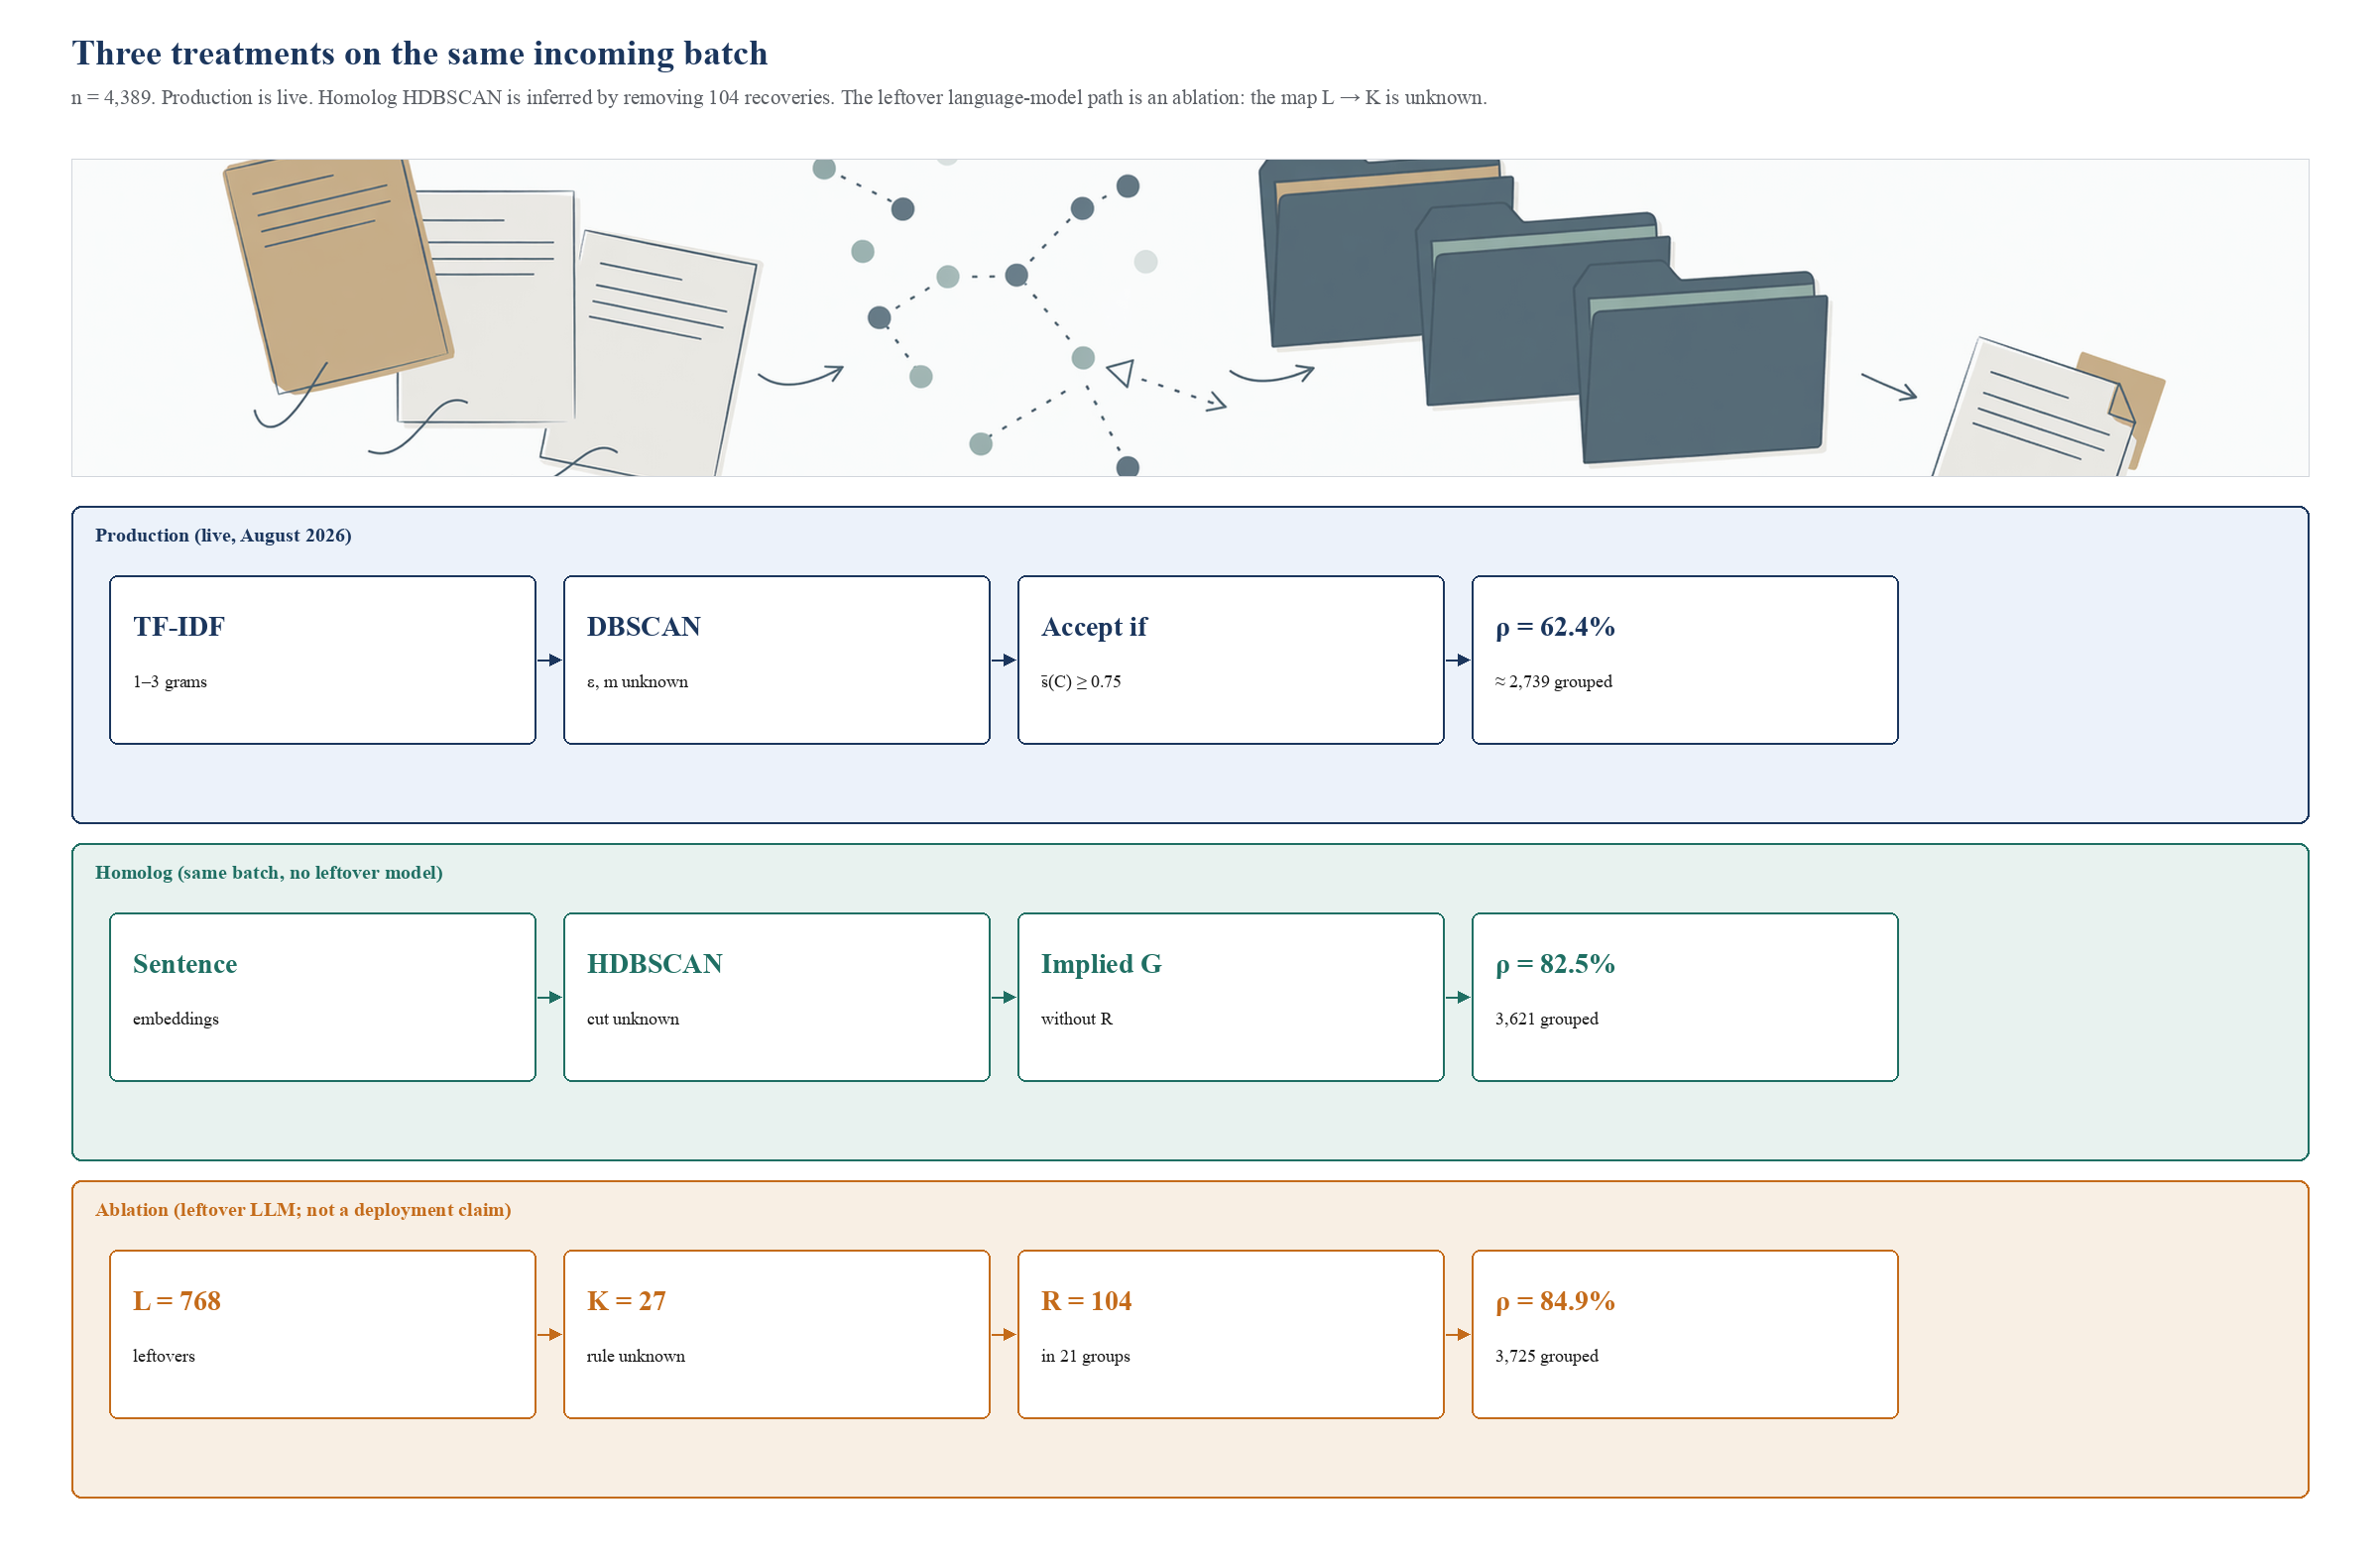
\includegraphics[width=\textwidth]{figures/fig1_pipeline.png}
\caption{Three treatments on the same incoming batch. Production is lexical. Homolog HDBSCAN is inferred by removing the 104 recoveries. The leftover language-model path is an ablation: the map $L\to K$ is unknown. Scene: Grok Imagine; stations and rates set in type.}
\label{fig:pipeline}
\end{figure*}

\begin{table}[t]
\caption{Experiment manifest. ``Unknown'' means the team note does not record the value. A later frozen run must fill every unknown cell before the homolog stack is treated as reproducible.}
\label{tab:manifest}
\small
\begin{tabular}{lll}
\toprule
Item & Production & Homolog \\
\midrule
Batch size & 4{,}389 (same set) & 4{,}389 \\
Batch window / checksum & Unknown & Unknown \\
Encoder & TF-IDF, 1--3 grams~\cite{salton1988term} & Sentence-Transformers, name unknown \\
Vector norm & $L_2$ & Unknown \\
Clusterer & DBSCAN~\cite{ester1996dbscan} & HDBSCAN~\cite{campello2013hdbscan,mcinnes2017hdbscan} \\
Radius / min.\ cluster size & Unknown & Unknown \\
Acceptance rule & Mean pairwise cosine $\ge 0.75$ & Unknown if the same cut applies \\
Language model & None & DeepSeek R1; date, prompt, host unknown \\
Candidate rule & --- & Unknown ($768 \rightarrow 27$) \\
Software pin & Unknown & Worker later loaded ST 5.1.2 vs.\ model 5.4.0 \\
Hardware / seed & Unknown & Embed step $\approx 3$ min on $\approx 4{,}000$ texts \\
Officer gold & None & None \\
\bottomrule
\end{tabular}
\end{table}

\subsection{Production stack (TF-IDF + DBSCAN)}

Each complaint is a document. The encoder is TF-IDF over unigrams, bigrams, and trigrams~\cite{salton1988term}. Vectors are $L_2$-normalized. DBSCAN then groups points that share a neighborhood of a given radius~\cite{ester1996dbscan}. After clustering, a group is accepted only if mean pairwise cosine similarity inside the group is at least 0.75.

Similarity is not transitive. $A$ can sit close to $B$, $B$ to $C$, and $C$ to $D$, while $A$ and $D$ score near 0.006 and still share a label. A later check uses distance to the cluster centroid, as a $z$-score, to flag intruders. That check behaved better on sentence embeddings than on TF-IDF.

\subsection{Homolog stack (embeddings + HDBSCAN)}

Encode each complaint with a Sentence-Transformers model~\cite{reimers2019sbert}. Cluster with HDBSCAN~\cite{campello2013hdbscan}. The checkpoint name is not in this file. Portuguese models such as BERTimbau exist~\cite{souza2020bertimbau}; naming one of them would be a guess.

\subsection{Leftover language-model pass (ablation, not a deployment claim)}

The team sent a reduced leftover list to DeepSeek R1 and counted 104 recoveries in 21 groups. Because the candidate rule and the hosting path are unknown, this pass is reported as an ablation and is withdrawn from the operational claim. A later run that sends leftover text off-site needs a written Ouvidoria basis, a retention limit, and a log of what left the building.

\subsection{Provisional review queues}

Grouped items are shown in three queues (Figure~\ref{fig:bands}): green (suggested bulk linking), yellow (officer confirms), and red (officer reads with care). A cluster at 100\% internal similarity means the texts are identical. About 87\% of grouped homolog items sat in green. If that queue were trusted, the remaining 13\% of $3{,}725$ would be about 484 complaints. That 484 is an arithmetic remainder. It is not officer minutes, and the band cut itself is not in the note.

\begin{figure}[t]
\centering
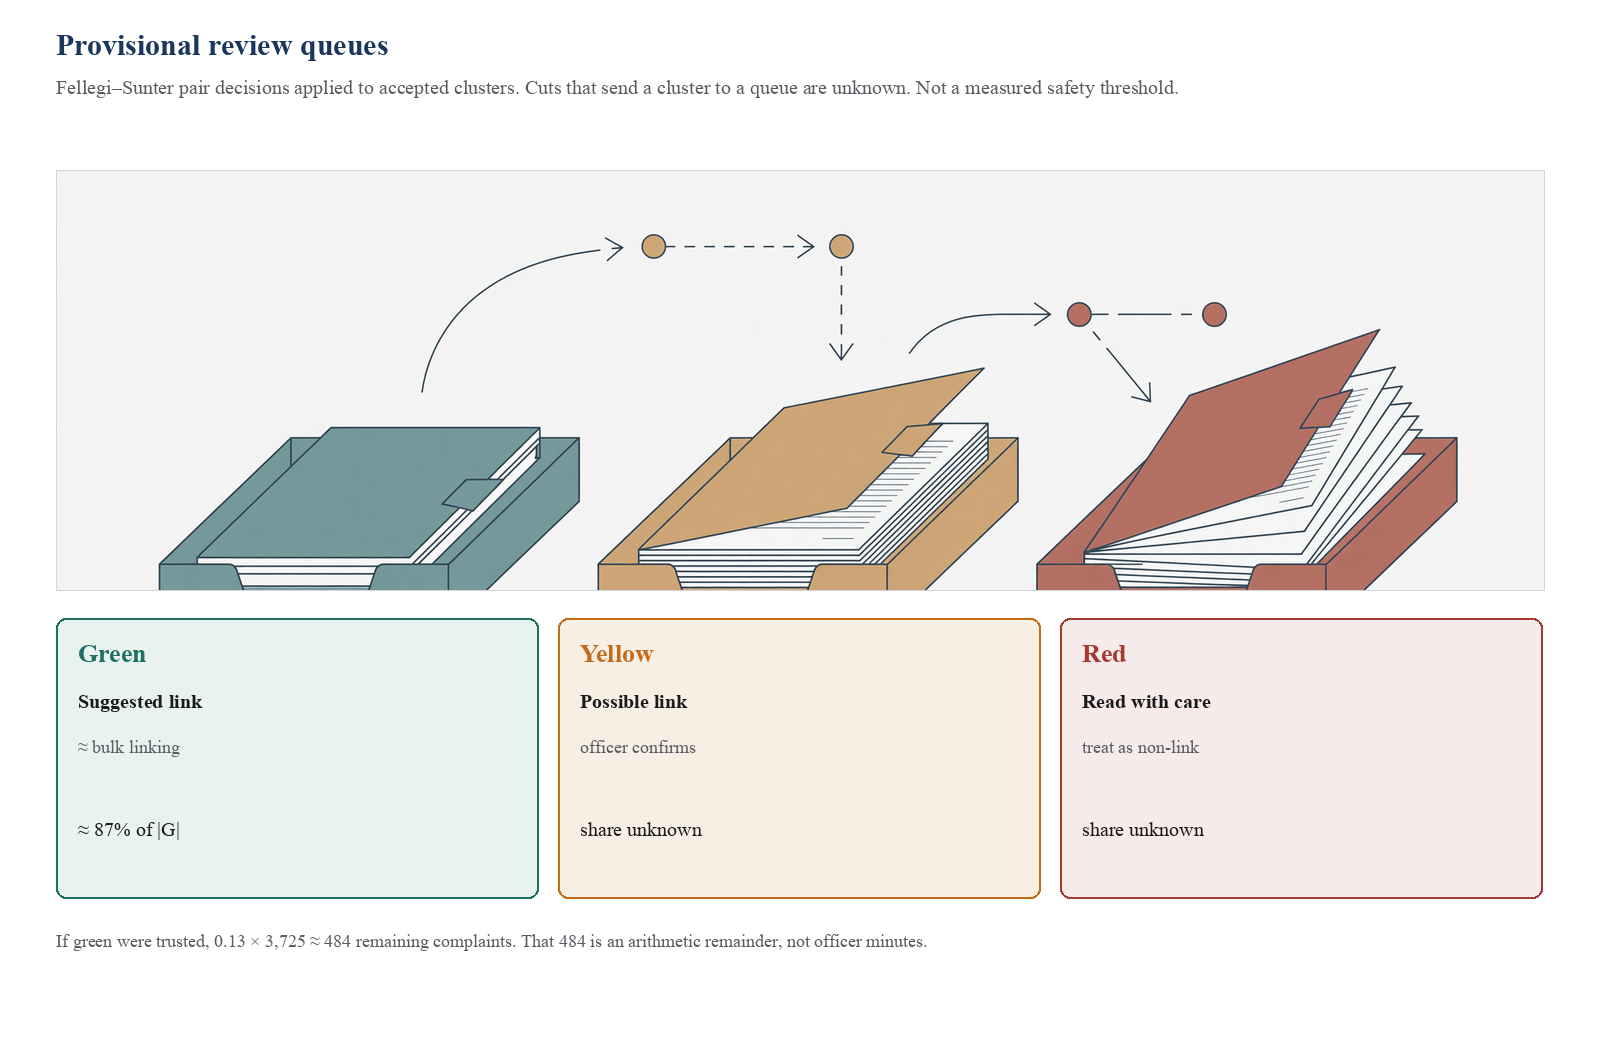
\includegraphics[width=\columnwidth]{figures/fig_bands.png}
\caption{Provisional review queues mapped to Fellegi--Sunter pair decisions. The cuts that send a cluster to a queue are not in the team note. Scene: Grok Imagine; queue labels set in type.}
\label{fig:bands}
\end{figure}

\section{Results}

\subsection{Three treatments, one batch}

Figure~\ref{fig:rate} and Table~\ref{tab:rates} split what v0.3 still printed as one jump.

\begin{figure}[t]
\centering
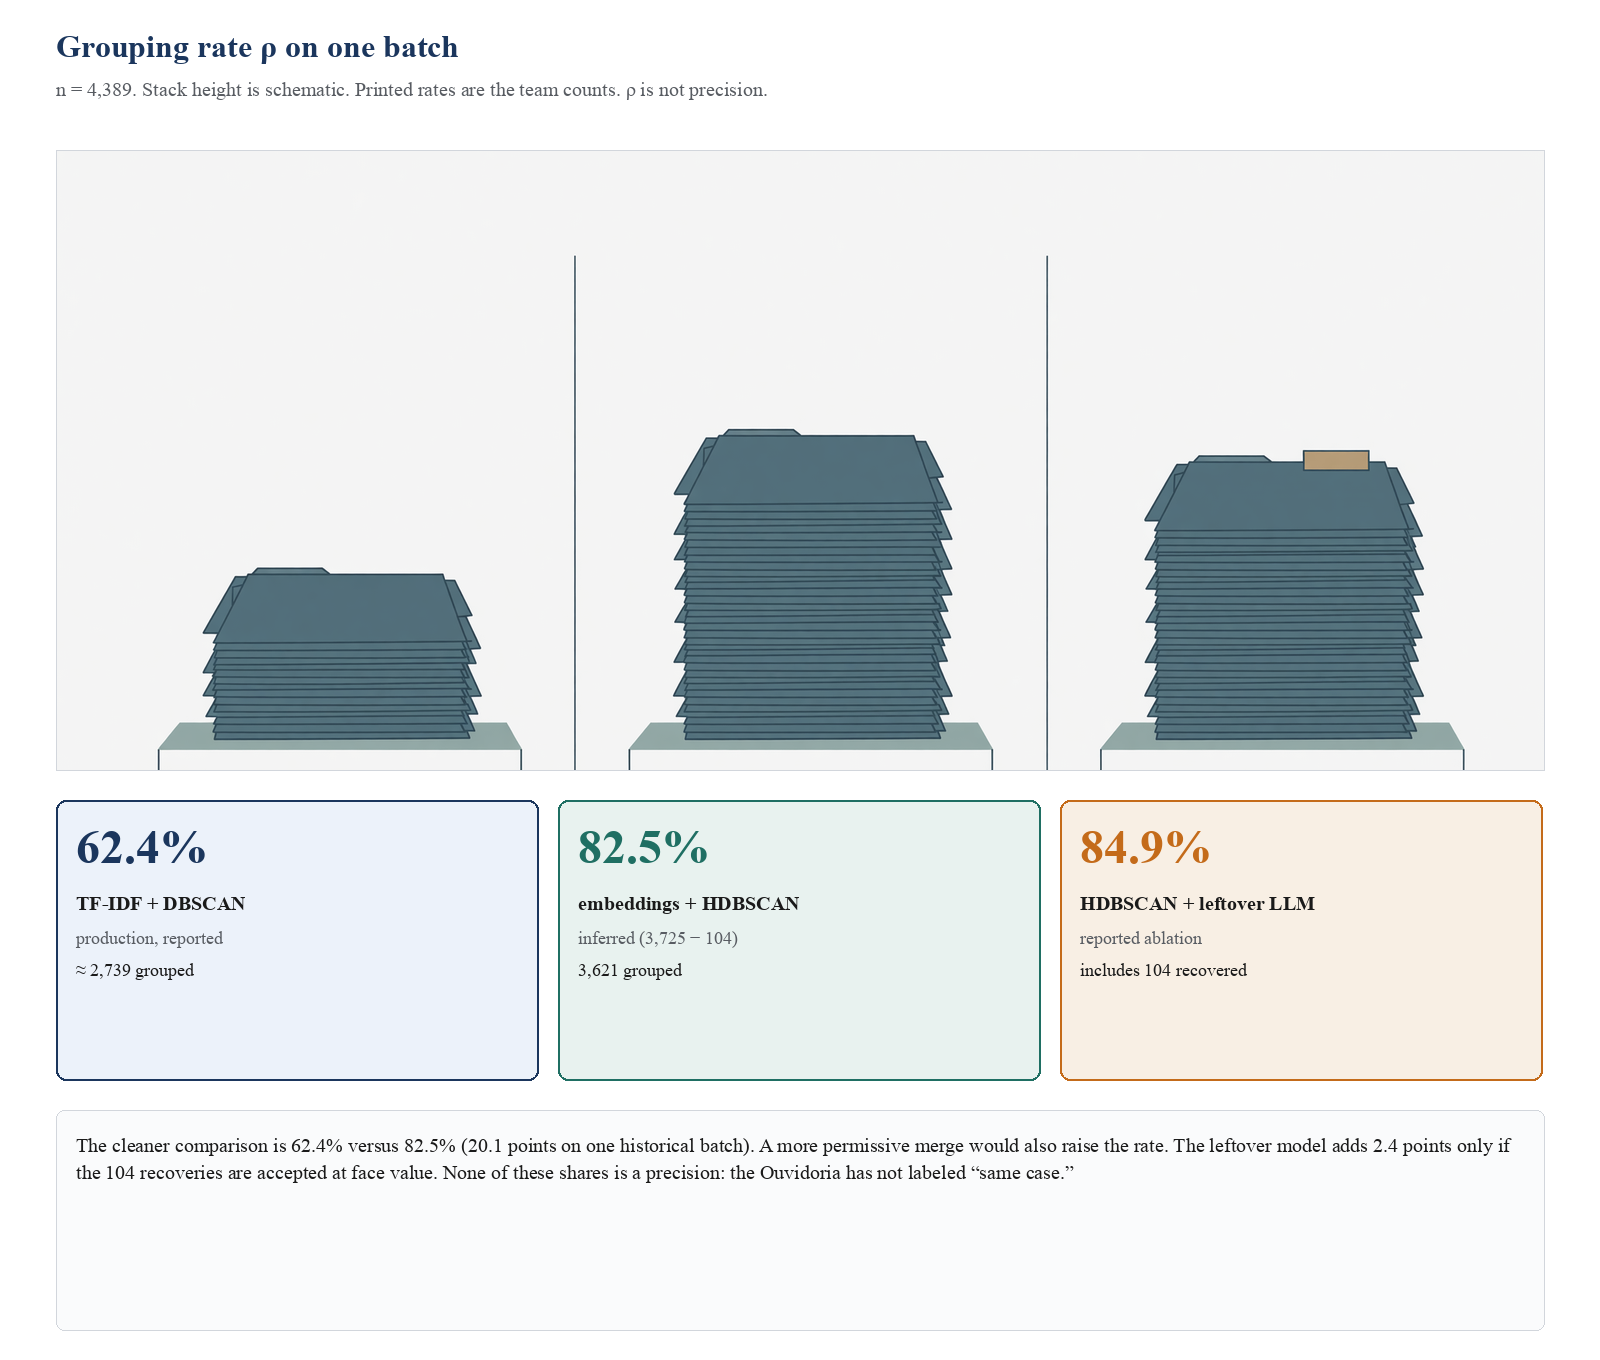
\includegraphics[width=0.92\columnwidth]{figures/fig2_grouping_rate.png}
\caption{Grouping rate $\rho$ on the same 4{,}389 complaints. Folder stacks are schematic. Printed rates are the team counts. The middle value is inferred ($3{,}725-104$). None of the rates is a precision.}
\label{fig:rate}
\end{figure}

\begin{table}[t]
\caption{Grouping rates on the 4{,}389-complaint batch. The last column is not precision.}
\label{tab:rates}
\begin{tabular}{llr}
\toprule
Treatment & What the note supports & Grouped \\
\midrule
TF-IDF + DBSCAN & Production stack, live in August 2026 & 62.4\% \\
Embeddings + HDBSCAN & Implied by removing 104 recoveries & 82.5\% \\
HDBSCAN + leftover LLM & Reported homolog total; filter unknown & 84.9\% \\
\bottomrule
\end{tabular}
\end{table}

The cleaner comparison is 62.4\% versus 82.5\%. That is still only a grouping-rate gap of 20.1 percentage points on one historical batch. A more permissive merge would also raise the rate. The leftover language model adds 2.4 points only if the 104 recoveries are accepted at face value.

The leftover path is in Figure~\ref{fig:funnel}: $768 \rightarrow 27 \rightarrow 104$ in 21 groups the team called themes.

\begin{figure}[t]
\centering
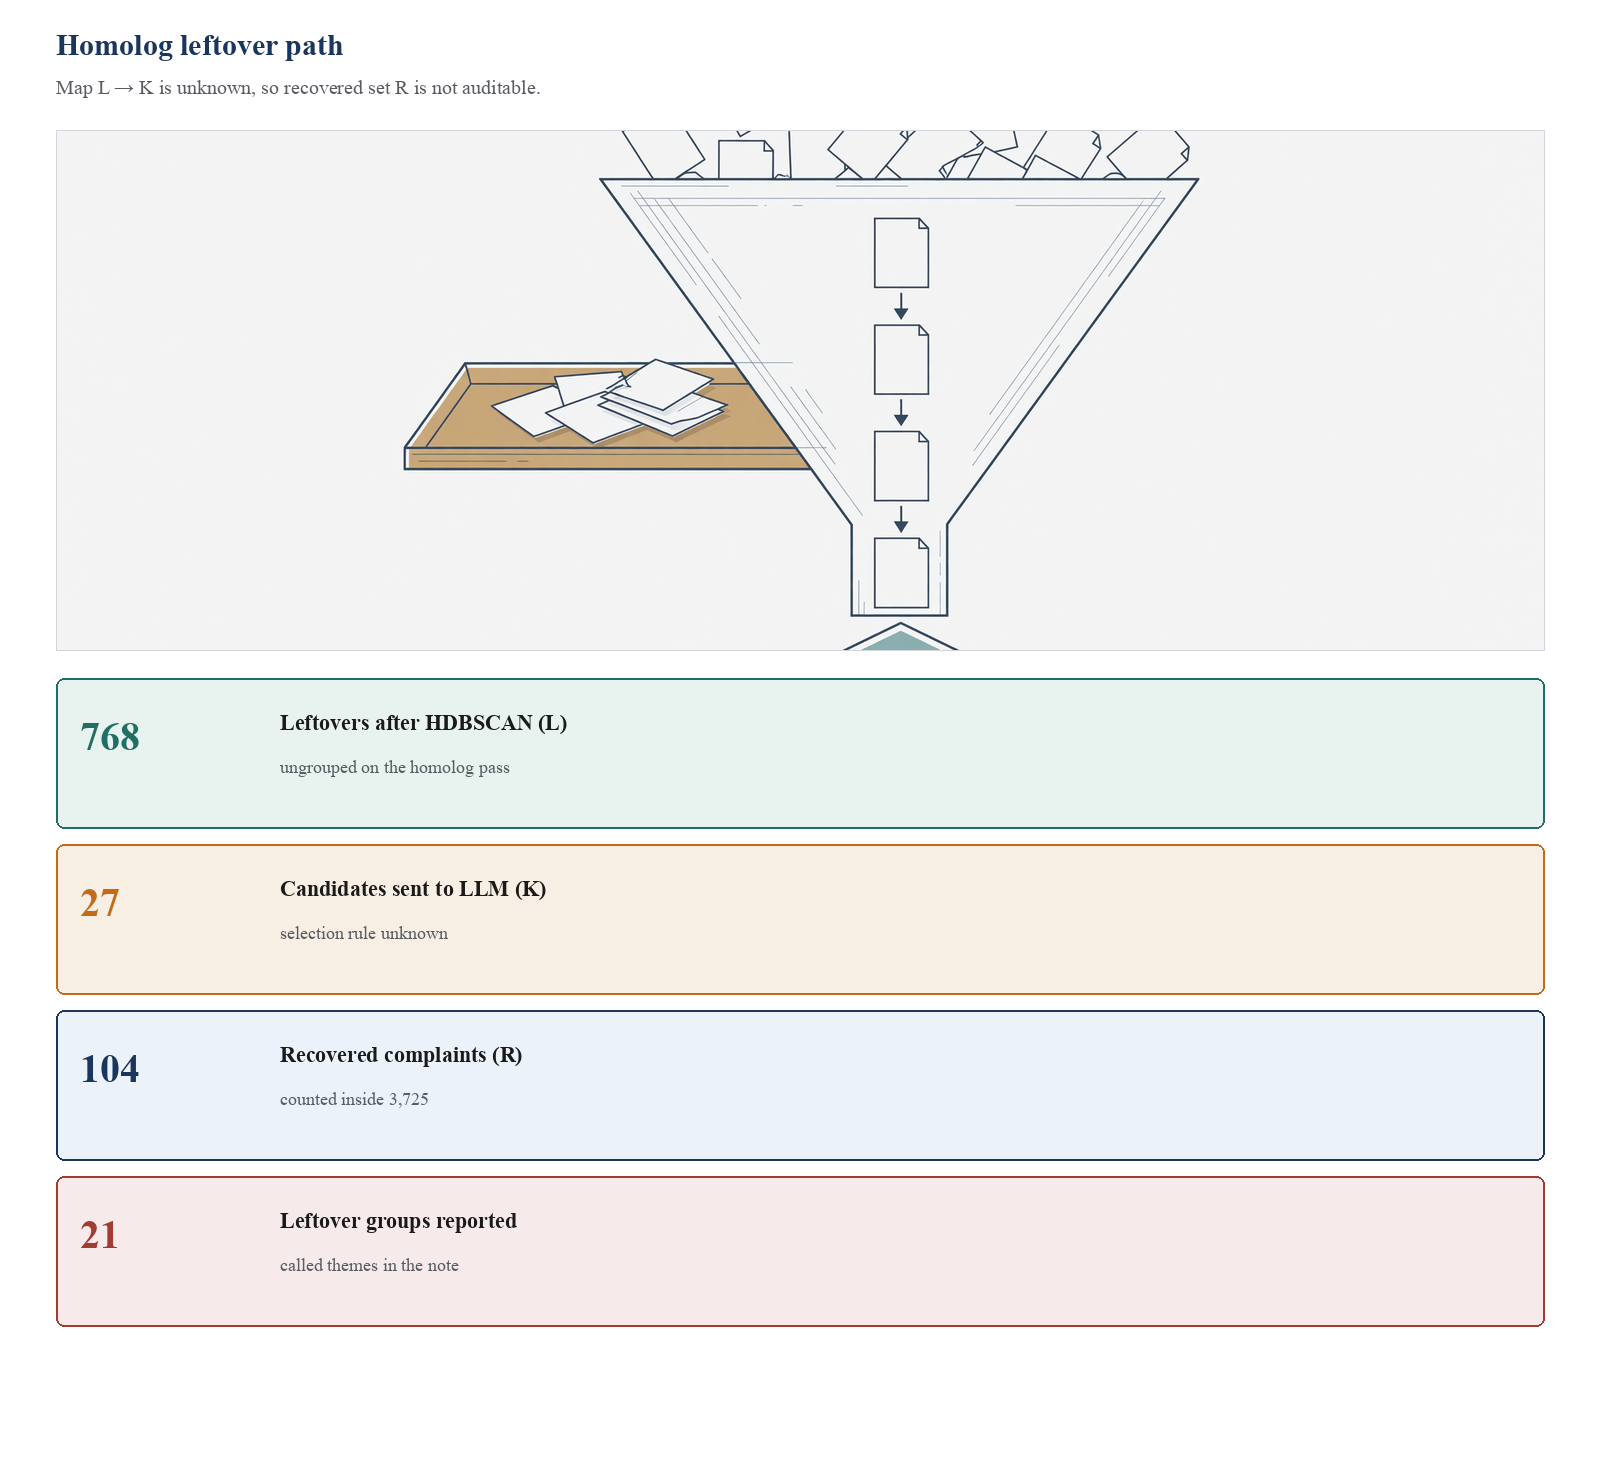
\includegraphics[width=\columnwidth]{figures/fig3_outlier_funnel.png}
\caption{Homolog leftover path. Counts typeset from the team note: $768 \rightarrow 27 \rightarrow 104$ in 21 groups. The selection rule for the 27 is unknown, so the 104 cannot yet be audited.}
\label{fig:funnel}
\end{figure}

\subsection{One production day}

The live TF-IDF job on 28 August 2026 shows what lexical clustering does when a wave arrives (Figure~\ref{fig:day}). At 08:00, 48 of 49 complaints sat in one cluster (mean similarity 85.68\%). At 12:00, 73 of 78 sat in a cluster of identical texts. The day total was 127 processed, 124 grouped (97.6\%), 3 leftovers.

A 97.6\% grouping rate on a campaign day is not in conflict with 62.4\% on the long set. The long set mixes ordinary days and waves. 28 August was a wave day.

\begin{figure*}[t]
\centering
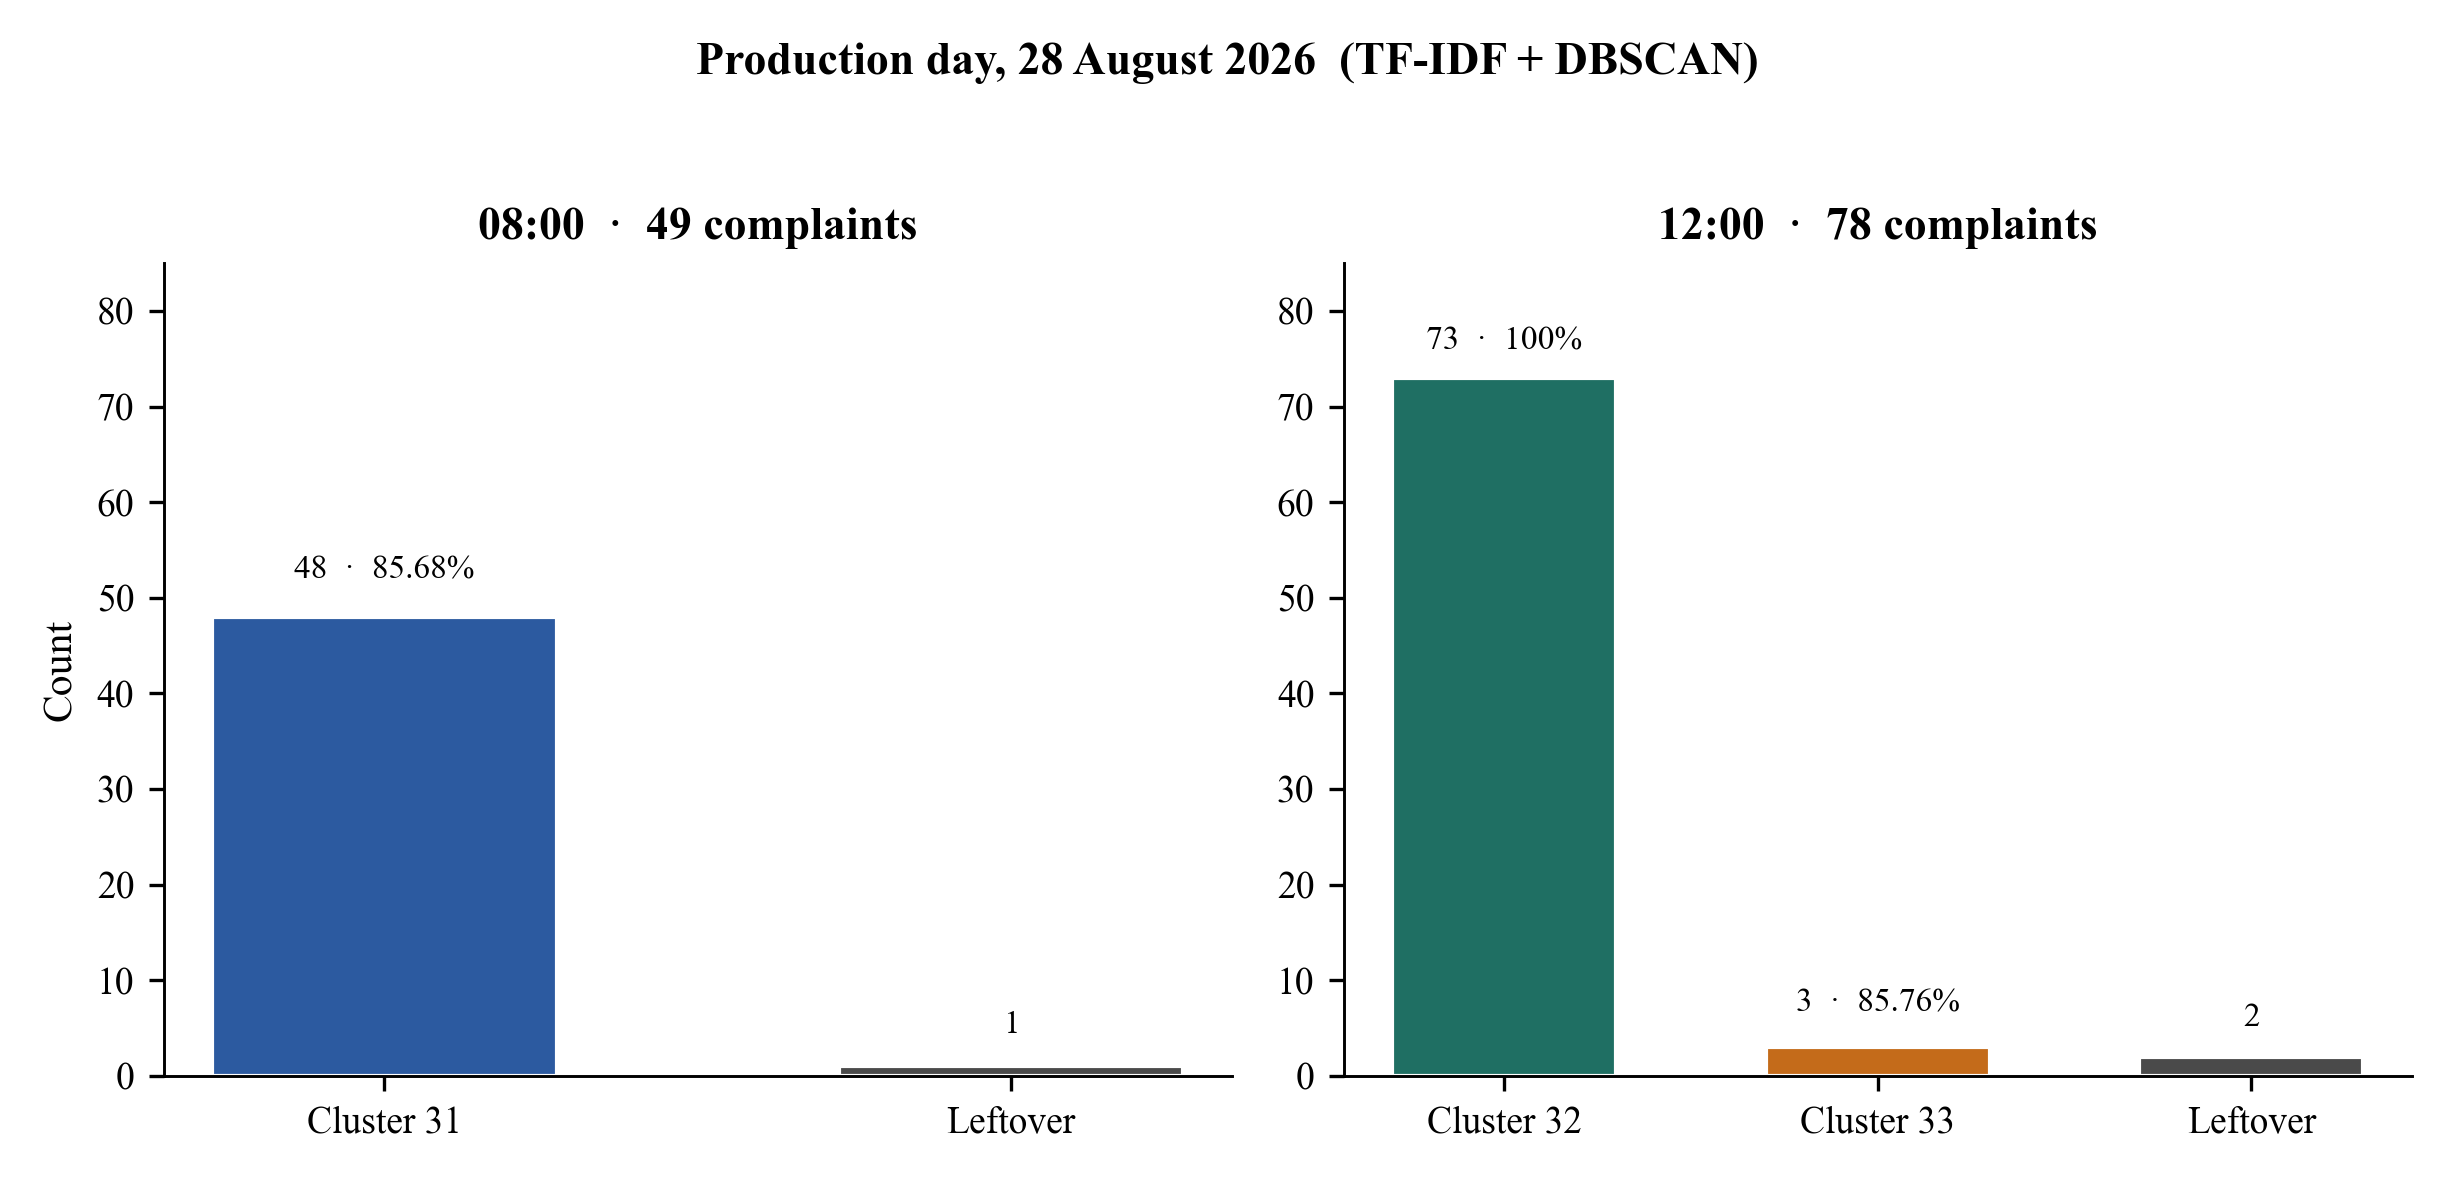
\includegraphics[width=0.92\textwidth]{figures/fig5_production_day.png}
\caption{Production TF-IDF + DBSCAN on 28 August 2026. Large clusters read as copy-paste or light paraphrase, not as ordinary mixed traffic.}
\label{fig:day}
\end{figure*}

\subsection{The same rule on public clustering sets}
\label{sec:public}

The Cear\'{a} batch has no officer gold. We do not invent one. We downloaded five public packs, ran the production rule on the texts, and wrote every count from that run into \texttt{experiments/public\_benchmarks.json}. Encoder: TF-IDF, 1--3 grams, $L_2$. Clusterer: DBSCAN on cosine distance, $\varepsilon=1-\tau=0.25$, $\mathrm{minPts}=2$. Keep a cluster only if mean pairwise cosine $\ge 0.75$. That $\varepsilon$ is the probe radius. It is not the missing Cear\'{a} radius. No complaint text left CGE. Events~2012 was not run: this machine has no Twitter token to hydrate tweet ids~\cite{mcminn2013events}.

Three packs are theme gold: 720 posts from six groups of 20~Newsgroups~\cite{lang1995newsweeder}; all 2{,}225 BBC News articles~\cite{greene2006bbc}; 1{,}510 single-topic Reuters-21578 wires from the eight largest remaining topics, at most 200 per topic, seed 20260925~\cite{lewis1997reuters}. Two packs are duplicate-question gold: 2{,}225 Quora questions from duplicate=1 pairs in the GLUE QQP train file, taking connected components until that $n$~\cite{wang2018glue}; 1{,}901 webmaster questions that sit in a CQADupStack duplicate component (MTEB mirror of Hoogeveen et al.)~\cite{hoogeveen2015cqadupstack}.

Figure~\ref{fig:public} and Table~\ref{tab:public} are those measured scores. On the three theme packs, $\rho$ is 3.2\%, 17.0\%, and 10.5\%. BCubed precision against the topic label stays near 1; recall stays below 0.01. The cut almost never rebuilds a newsgroup, a BBC desk, or a Reuters topic. On Quora duplicates it grouped 899 of 2{,}225 ($\rho=40.4\%$) in 301 clusters; BCubed $F_1$ against the pair components was 0.13, because those components are large paraphrase chains and the lexical cut only keeps the tight copies. On CQADupStack webmasters it grouped 21 of 1{,}901 ($\rho=1.1\%$) in 10 clusters; BCubed precision was 0.998 and $F_1$ was 0.42.

A 0.75 lexical cut is Broder's job. It is not Lang's, Greene's, or Lewis's topic partition. It also does not recover a loose duplicate-question family.

\begin{figure}[t]
\centering
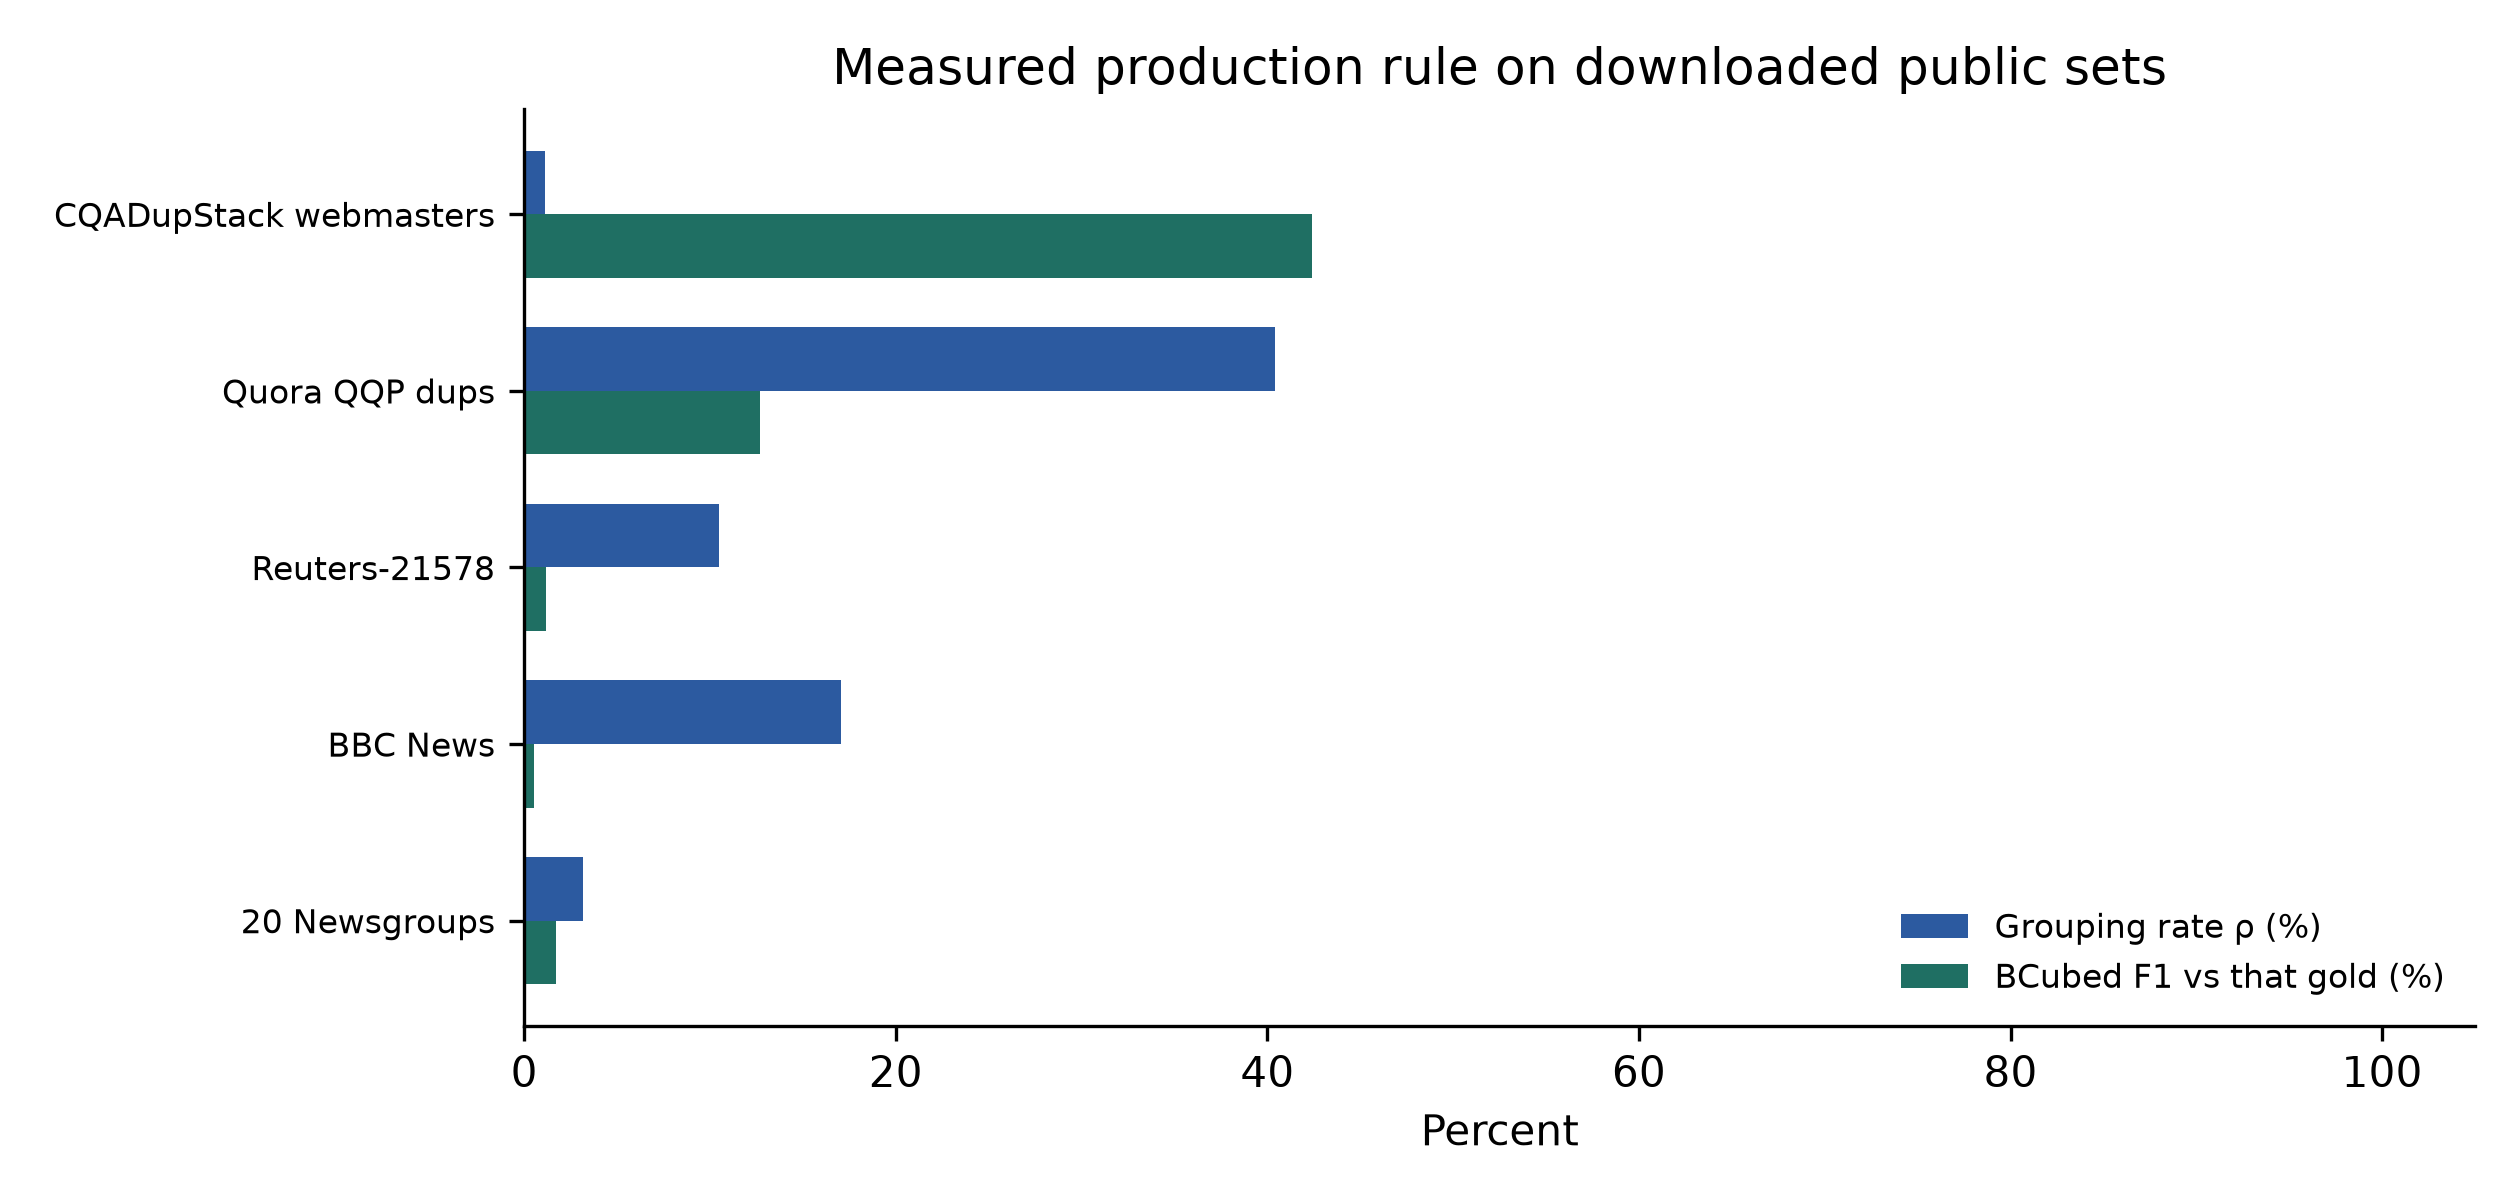
\includegraphics[width=\columnwidth]{figures/fig6_public_benchmarks.png}
\caption{Measured production rule on the five downloaded packs. Theme gold on the left-hand jobs; duplicate-question gold on Quora and CQADupStack. $\rho$ is still not a Cear\'{a} precision.}
\label{fig:public}
\end{figure}

\begin{table}[t]
\caption{Measured production rule. Every cell comes from \texttt{experiments/public\_benchmarks.json}. BCubed is against that pack's gold, not against a COUVI officer. $\varepsilon=0.25$.}
\label{tab:public}
\small
\begin{tabular}{lrrrrr}
\toprule
Pack (gold) & $n$ & $\rho$ & Clusters & BCubed $P$ & BCubed $F_1$ \\
\midrule
20 Newsgroups (theme) & 720 & 3.2\% & 10 & 1.00 & 0.02 \\
BBC News (theme) & 2{,}225 & 17.0\% & 189 & 1.00 & 0.01 \\
Reuters-21578 (theme) & 1{,}510 & 10.5\% & 73 & 1.00 & 0.01 \\
Quora QQP dups & 2{,}225 & 40.4\% & 301 & 0.99 & 0.13 \\
CQADupStack webmasters & 1{,}901 & 1.1\% & 10 & 1.00 & 0.42 \\
\bottomrule
\end{tabular}
\end{table}

\subsection{Laboratory generic stacks (product unchanged)}
\label{sec:generic}

The Ouvidoria rule stays in production. For the paper we also ran task-aware laboratory stacks on the same five packs. Script: \texttt{experiments/run\_generic\_benchmarks.py}. Encoder: \texttt{sentence-transformers/all-MiniLM-L6-v2}~\cite{reimers2019sbert}. Theme packs use KMeans with $k$ equal to the number of gold classes. Duplicate-question packs use HDBSCAN with $\mathrm{min\_cluster\_size}=2$. No CGE complaint text. No change to Airflow or to the TF-IDF + DBSCAN job.

Figure~\ref{fig:generic} and Table~\ref{tab:generic} compare BCubed $F_1$ against each pack's gold. On theme gold the laboratory stack lifts $F_1$ from near zero to 0.67 (20~Newsgroups), 0.92 (BBC), and 0.73 (Reuters). On duplicate-question gold it lifts Quora from 0.13 to 0.46 and CQADupStack webmasters from 0.42 to 0.58. Those gains are for other golds. They are not a licence to replace the Cear\'{a} production cut.

\begin{figure}[t]
\centering
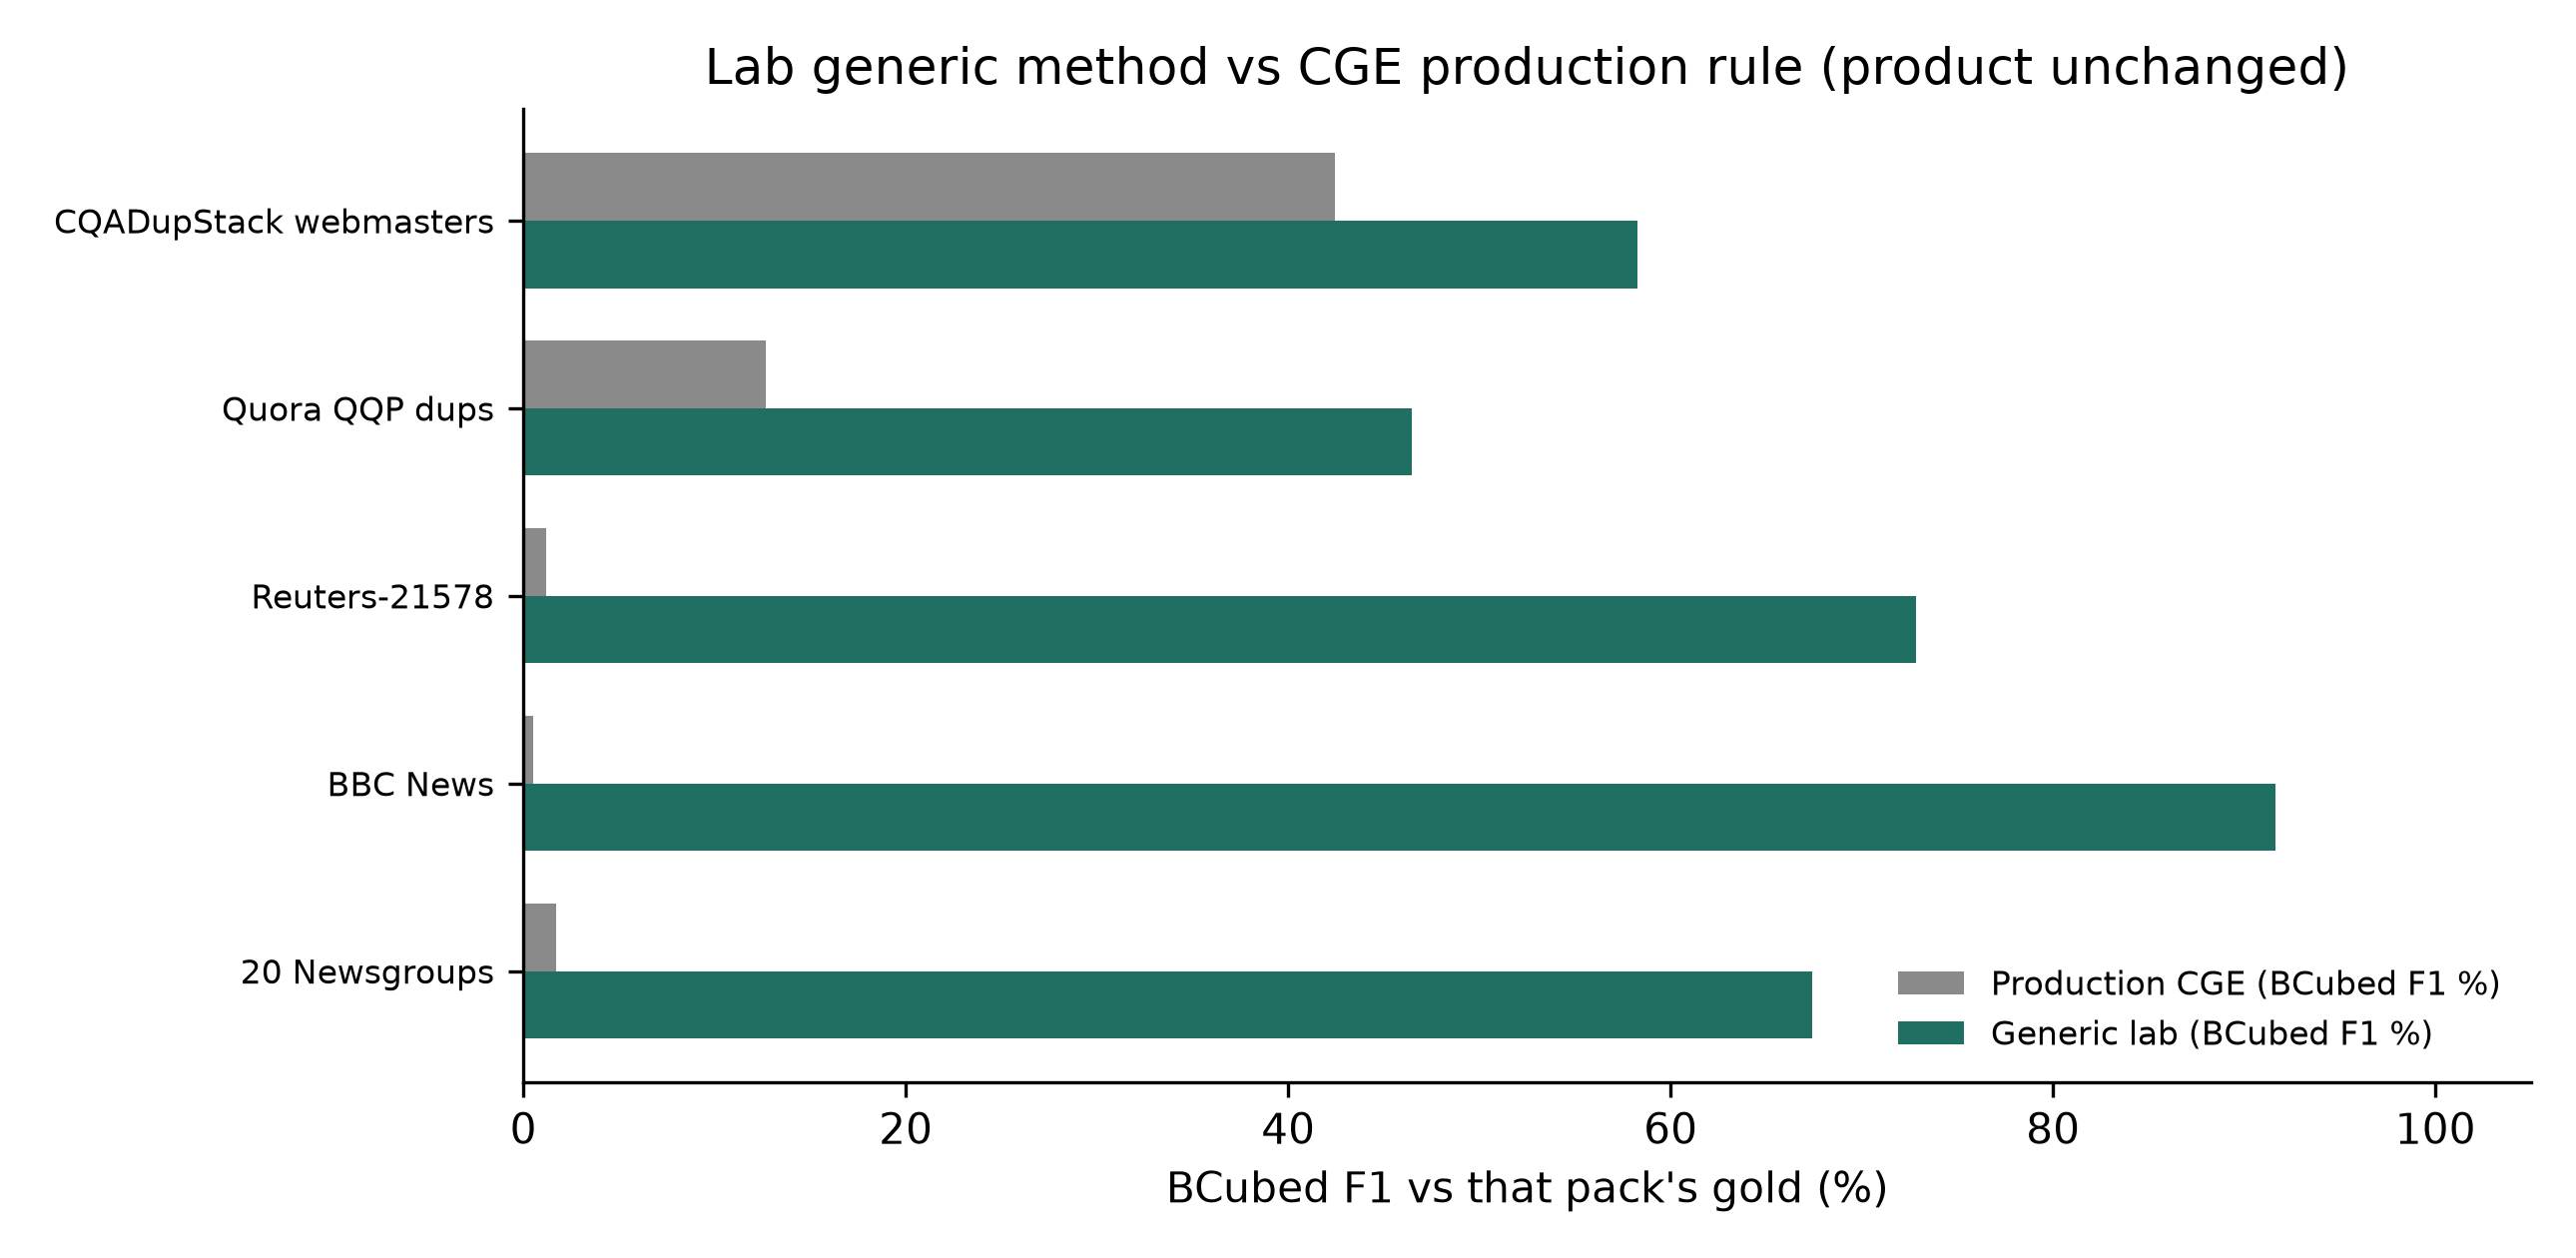
\includegraphics[width=\columnwidth]{figures/fig7_generic_vs_production.png}
\caption{Measured BCubed $F_1$ on the same five packs. Grey: CGE production rule. Teal: laboratory generic stack. The Ouvidoria product is unchanged.}
\label{fig:generic}
\end{figure}

\begin{table}[t]
\caption{Measured BCubed $F_1$ on downloaded packs. Production = TF-IDF + DBSCAN ($\tau=0.75$). Generic theme = MiniLM + KMeans($k$). Generic duplicate = MiniLM + HDBSCAN. Source: \texttt{experiments/generic\_benchmarks.json}.}
\label{tab:generic}
\small
\begin{tabular}{lrrr}
\toprule
Pack (gold) & $n$ & Prod.\ $F_1$ & Generic $F_1$ \\
\midrule
20 Newsgroups (theme) & 720 & 0.02 & 0.67 \\
BBC News (theme) & 2{,}225 & 0.01 & 0.92 \\
Reuters-21578 (theme) & 1{,}510 & 0.01 & 0.73 \\
Quora QQP dups & 2{,}225 & 0.13 & 0.46 \\
CQADupStack webmasters & 1{,}901 & 0.42 & 0.58 \\
\bottomrule
\end{tabular}
\end{table}

\subsection{What broke after the test}

September 2026 showed the gap between a homolog notebook and a daily Airflow job. A homolog build of the new stack failed and later recovered. The live grouping collapsed toward one cluster and many leftovers. Infrastructure blocked Python library downloads. The Airflow worker loaded Sentence-Transformers 5.1.2 against a model saved with 5.4.0. Short texts carried little signal, and cosine grouping then failed. So 82.5\% and 84.9\% are batch results. They are not the steady daily rate.

\section{Human validation protocol (unrun)}

No COUVI officer has labeled this batch. The protocol below is what v0.5 must run. It is not a result.

\paragraph{Unit.} A pair or a cluster is \emph{same event} when a reasonable officer would open one case file. \emph{Related theme} means the same subject without the same event. \emph{Different} and \emph{unclear} are the other two codes.

\paragraph{Sample.} Stratify. About 50 green clusters, 30 yellow, 20 red, 40 leftovers, and 30 pairs drawn from clusters larger than 20. Include short texts (under 20 tokens) as their own stratum if the log can list them. Two officers, blinded to stack and to each other. A third officer adjudicates disagreements.

\paragraph{Metrics.} Pairwise precision of proposed merges; false-merge and false-split rates; Cohen's $\kappa$; BCubed precision and recall against the adjudicated clustering~\cite{amigo2009bcubed}. Report each treatment separately: production, HDBSCAN, HDBSCAN plus leftover model---and only after the leftover filter is written down.

\paragraph{Workload.} If the queues go into a live week, log accept, reject, split, and minutes per 100 complaints. Until those minutes exist, do not call 484 an officer load.

\section{Discussion}

Lexical clustering already catches the easy wave: identical or near-identical paste. That is useful on a morning like 28 August. It is the wrong tool when two people write the same event in different words.

The public probe in Section~\ref{sec:public} is the control that the Cear\'{a} note could not run. A 0.75 lexical cut almost never reconstructs a newsgroup, a BBC desk, or a Reuters topic. On labeled duplicate questions it either stays almost silent (CQADupStack) or groups the tight copies and misses the paraphrase chain (Quora). That is evidence for the job split in Figure~\ref{fig:case}, not a precision on ombudsman files. Section~\ref{sec:generic} shows that a different laboratory stack can raise BCubed $F_1$ on those packs. That stack is not the Ouvidoria product.

The homolog HDBSCAN step moves the cut from tokens to sense. Rabbi et al.\ needed a time window and identity keys to call two consumer texts a duplicate~\cite{rabbi2026duplicate}. Similaridade does not yet use those keys. That is a gap, not a virtue: a 30-day window and an agency field would be the first cheap control on short texts.

The leftover language-model pass follows the cost lesson in Rakhimzhanov et al.~\cite{rakhimzhanov2025transport}---spend the expensive model on leftovers---but the $768 \rightarrow 27 \rightarrow 104$ funnel is not yet a result. If the 27 candidates were chosen by a person who already saw the 104, the credit is circular.

Compared with Silva et al.~\cite{silva2026bridging} and Tang et al.~\cite{tang2024bertopic}, the claim here is not a new router and not a dashboard of themes. It is a count of how many ombudsman files the machine put in a group before a human reads them. Fellegi and Sunter gave the pair decision~\cite{fellegi1969linkage}. Broder gave resemblance for pages~\cite{broder1997resemblance}. The ombudsman pile is shorter, in Portuguese, and closed by a stamp.

\section{Limitations}

The limits are part of the result.
\begin{enumerate}
\item Counts come from team reports, not from a frozen public extract of \texttt{etl.similaridade\_log}.
\item There is no officer gold on the Cear\'{a} batch. BCubed in Table~\ref{tab:public} is against the gold of each downloaded pack, not against a COUVI stamp. Events~2012 was not run.
\item The embedding checkpoint, DBSCAN radius, HDBSCAN size, and band cuts are unknown.
\item The leftover language-model pass has an undocumented filter and an unstated host.
\item September failures show that the homolog rates are not the current daily truth.
\item We do not measure minutes saved for the officer or days saved for the citizen.
\item Authorship is incomplete.
\end{enumerate}

A submission without the protocol in Section~7, filled, will still read as a slide.

\section{Ethics and data}

Complaint text can identify a person or a public servant. This draft uses only counts. Any later replication package must stay inside CGE, with access logged, or use a redacted sample approved by the Ouvidoria.

The leftover pass used DeepSeek R1. The team note does not say whether that call stayed on a machine inside CGE. Until that path is written down, we do not treat the leftover pass as part of the production design. A later run that sends leftover text off-site needs a written Ouvidoria basis, a retention limit, a ban on provider training use, and a log of what left the building.

Clustering is an aid. An officer still closes the case. Linking two files that are not the same event can bury a second victim. That is why green stays a queue.

\section{Conclusion}

On 4{,}389 real complaints, TF-IDF + DBSCAN grouped 62.4\% of the texts. Embeddings + HDBSCAN grouped an inferred 82.5\% before any language model. A leftover pass then raised the reported share to 84.9\%, but the filter and the host of that pass are unknown, so that last step is not a deployment claim. A wave morning in August showed the lexical stack at work: 97.6\% grouped that day, almost all in two large clusters.

The next version needs what this draft cannot invent: COUVI labels on a stratified sample, a filled manifest, and a week of production logs after Airflow is stable. Until then the honest claim is smaller. The Ouvidoria already groups copy-paste waves. A semantic stack grouped more of the same historical batch. Daily production of that stack is still being earned.

\begin{acks}
ASESI colleagues who discussed the method in June--September 2026, including Leonardo Borba and Oton; the COUVI officers who will have to trust or reject the green queue; and Lucas Pimentel, who hosts the internal GitLab project. Errors in this draft are the authors'.
\end{acks}

\section*{CRediT (provisional)}
Methodology, software, and investigation (homolog measurements): Berg Silva. Team review: Charles and Ana Luiza Cruz. Conceptualization and writing (original draft): Francisco Nauber Bernardo Gois. Other roles to be assigned.

\section*{Funding}
No external grant. Work done as part of CGE-CE / ASESI operations.

\section*{Competing interests}
The authors work for the agency that operates the system. That is the point of a practice paper. It is also a conflict to declare.

\section*{Data availability}
Complaint text is not public. Aggregate figures can be checked against CGE internal logs by staff with access.

\section*{Use of AI tools}
A language model helped organize this English draft from team notes. Conceptual scenes were drawn with Grok Imagine (model grok-imagine-image-quality). Rates, counts, and captions were set in type from the team note; the generator was not asked to write numerals. The 28 August production-day chart remains matplotlib. No complaint text was sent to an image or language model. The corresponding author is responsible for every number.

\bibliographystyle{ACM-Reference-Format}
\bibliography{refs}

\end{document}
